\documentclass{article}

\usepackage{amsmath}
\usepackage{amsfonts}
\usepackage{multicol}
\usepackage{siunitx}
\usepackage{graphicx}
\usepackage{hyperref}
\usepackage{subcaption}
\usepackage{caption}
\usepackage{gensymb}
\usepackage{geometry}
\usepackage[nottoc,notlot,notlof]{tocbibind}
\usepackage{diffcoeff}
\usepackage{physics}
\usepackage{tabularx}
\usepackage[headings]{fullpage}

\newcolumntype{Y}{>{\centering\arraybackslash}X}


\usepackage{fancyhdr}
\pagestyle{fancy}
\fancyhf{}
\fancyhead[LE,RO]{\thepage}
\fancyhead[LO,RE]{\rightmark}

\newenvironment{Figure}{\par\medskip\noindent\minipage{\linewidth}}{\endminipage\par\medskip}
\setlength{\columnsep}{0.4in}
\linespread{1.5}


\title{7CCP4000 Project in Physics\\ 
	\huge \textbf{The Grotthuss Process}\\ }

\date{\today}
\author{Sebastian Budd\\Supervisor: Prof. Tony Paxton}


\begin{document}

  \pagenumbering{gobble}
  
  \maketitle

\begin{abstract}
The Grotthuss process, also known as proton jumping, is the movement of protons between molecules in bulk water; it underlies, amongst other things, the electrical conductivity of water and the transfer of charge in water wires inside biological molecules. Here we outline a method for modelling the Grotthuss process using Polarisable Ion Tight Binding. Molecular dynamics simulations are created to measure the rate of proton jumping and map it to the Arrhenius equation, finding the activation energy of a Grotthuss jump to be $0.1808 \pm 0.0496$ eV, and the rate at which a proton jumps from one molecule to another is found to be given by the formula $(2184.36 \pm 509.17)\exp{-\frac{2098.00 \pm 576.80}{T}} \text{ps}^{-1}$.
\end{abstract}
	
\newpage
\setcounter{page}{2}
\pagenumbering{arabic}

\tableofcontents

\newpage

\begin{multicols}{2}
\section{Introduction}

Water is a member of a small family of simple molecular substances that contain an abundance of hydrogen bonding, a phenomenon which causes atoms of different molecules to be very strongly attracted to each other. For a small proportion of water molecules this causes a phenomenon called autoprotonation, where one water molecule takes a proton from another water molecule, creating two ions: OH\textsuperscript{-} (hydroxide) and H\textsubscript{3}O\textsuperscript{+} (hydronium). 

The Grotthuss process relates to how positive charge moves throughout a body of water through protons moving from H\textsubscript{3}O\textsuperscript{+} to H\textsubscript{2}O repeatedly. This process underlies several important properties of water. In physics, it helps to explain its conductivity and how it varies with respect to temperature, and in biology governs the transfer of charge in water wires inside biological molecules.\cite{pomes1996structure}

Empirical tight binding was chosen as the model for simulating this process because of its successes in modelling hydrogen bonding in water and ice.\cite{Lozovoi2014} Notably for our simulation, it correctly predicts that hydrogen atoms lie almost in line with the hydrogen bond\footnote{O-H covalent bonds are offset from the hydrogen bonds by $5.5^{\circ}$.} and predicts the length of the hydrogen bond to be $5.34$ Bohr compared to the experimental value of $5.33$ Bohr.\cite{Lozovoi2014} Additionally, the model properly orders the relative densities of liquid water and ice. 

\section{Water, Hydroxide and Hydronium}
\subsection{Hydrogen Bonding}

Hydrogen bonding is a type of inter-molecular bonding that is much stronger than typical van der Waals forces, and systems containing them have unique properties.. It occurs in substances where a nitrogen, oxygen or fluorine atom is covalently bonded to hydrogen atom, and another molecule contains a lone pair of electrons. Nitrogen, oxygen and fluorine are so strongly electronegative that the hydrogen atom becomes positively charged and has an electrostatic attraction to lone pairs of electrons. 

Water molecules have two protons with large positive charges and two lone pairs in a tetrahedral structure, meaning that each molecule can hydrogen bond to four molecules around it.

\subsubsection{Covalent versus Ionic}
Hydrogen bonds display both ionic and covalent properties.\cite{Weinhold2014} In addition to the electrostatic force between the negatively charged oxygen atoms and positively charged hydrogen atoms, the molecules form weak covalent bonds with each other by sharing electrons. Electrons are transferred to the anti-bonding orbital of the covalently bonded OH pair. This causes the length of covalent bonds in liquid water to be slightly longer than in the gas phase, and the O-O distance to be roughly 15\% smaller than if just ionic properties were considered.\cite{Hbonding}

\subsection{Autoprotonation}
\label{sec:autoprotonation}
Water molecules in liquid water undergo the reversible reaction
\begin{equation}
	2\text{H}_{2}\text{O} \leftrightarrow \text{H}_{3}\text{O}^{+} + \text{OH}^{-}
\end{equation}
and so, due to Le Chatelier's principle,\cite{le1898limits} a small number of hydroxide and hydronium ions exist in liquid water.

The number of ions in pure water is calculated using the formula for the pH,
\begin{equation}
	\textrm{pH}=-\textrm{log}_{10}(a_{H^+})
\end{equation}
where $a_{H^{+}}$ is the hydrogen ion activity. In water, this is equal to the molar concentration $[H^{+}]$ which is in turn equal to the molar concentration of hydronium ion $[H_{3}0^{+}]$.\footnote{This is due to the fact that lone protons cannot exist in liquid water.\cite{bell2013proton}} We can rearrange this to 
\begin{equation}
	a_{H^+} = 10^{-\textrm{pH}}
\end{equation}
The pH of water at room temperature and pressure (RTP) is 7, and therefore $[H_{3}0^{+}] = 10^{-7}\text{mol}/L$. 

This means that at RTP, the number of hydronium ions in a litre of water is $6.022 \times 10^{16}$ and by dividing the number of molecules in a litre of water by this number, we find that in RTP water, one in every $5.5508\times10^{8}$ molecules is a hydronium ion.
\subsection{Unique Properties}
\subsubsection{High Melting and Boiling Points}
Hydrogen bonding means that the intermolecular forces in water are very strong, resulting in melting and boiling points for water being much higher than other analogous molecules. For instance, H\textsubscript{2}S has melting and boiling points of $-82^{\circ}$C and $-60^{\circ}$C respectively.
\subsubsection{Ice}
The fact that water molecules have two protons and two lone pairs of electrons means that water molecules can arrange themselves into a very ordered crystal lattice, whereby the oxygen atoms arrange themselves into a tetrahedral structure similar to diamond. Each water molecule is hydrogen bonded to four other water molecules.

\begin{Figure}
	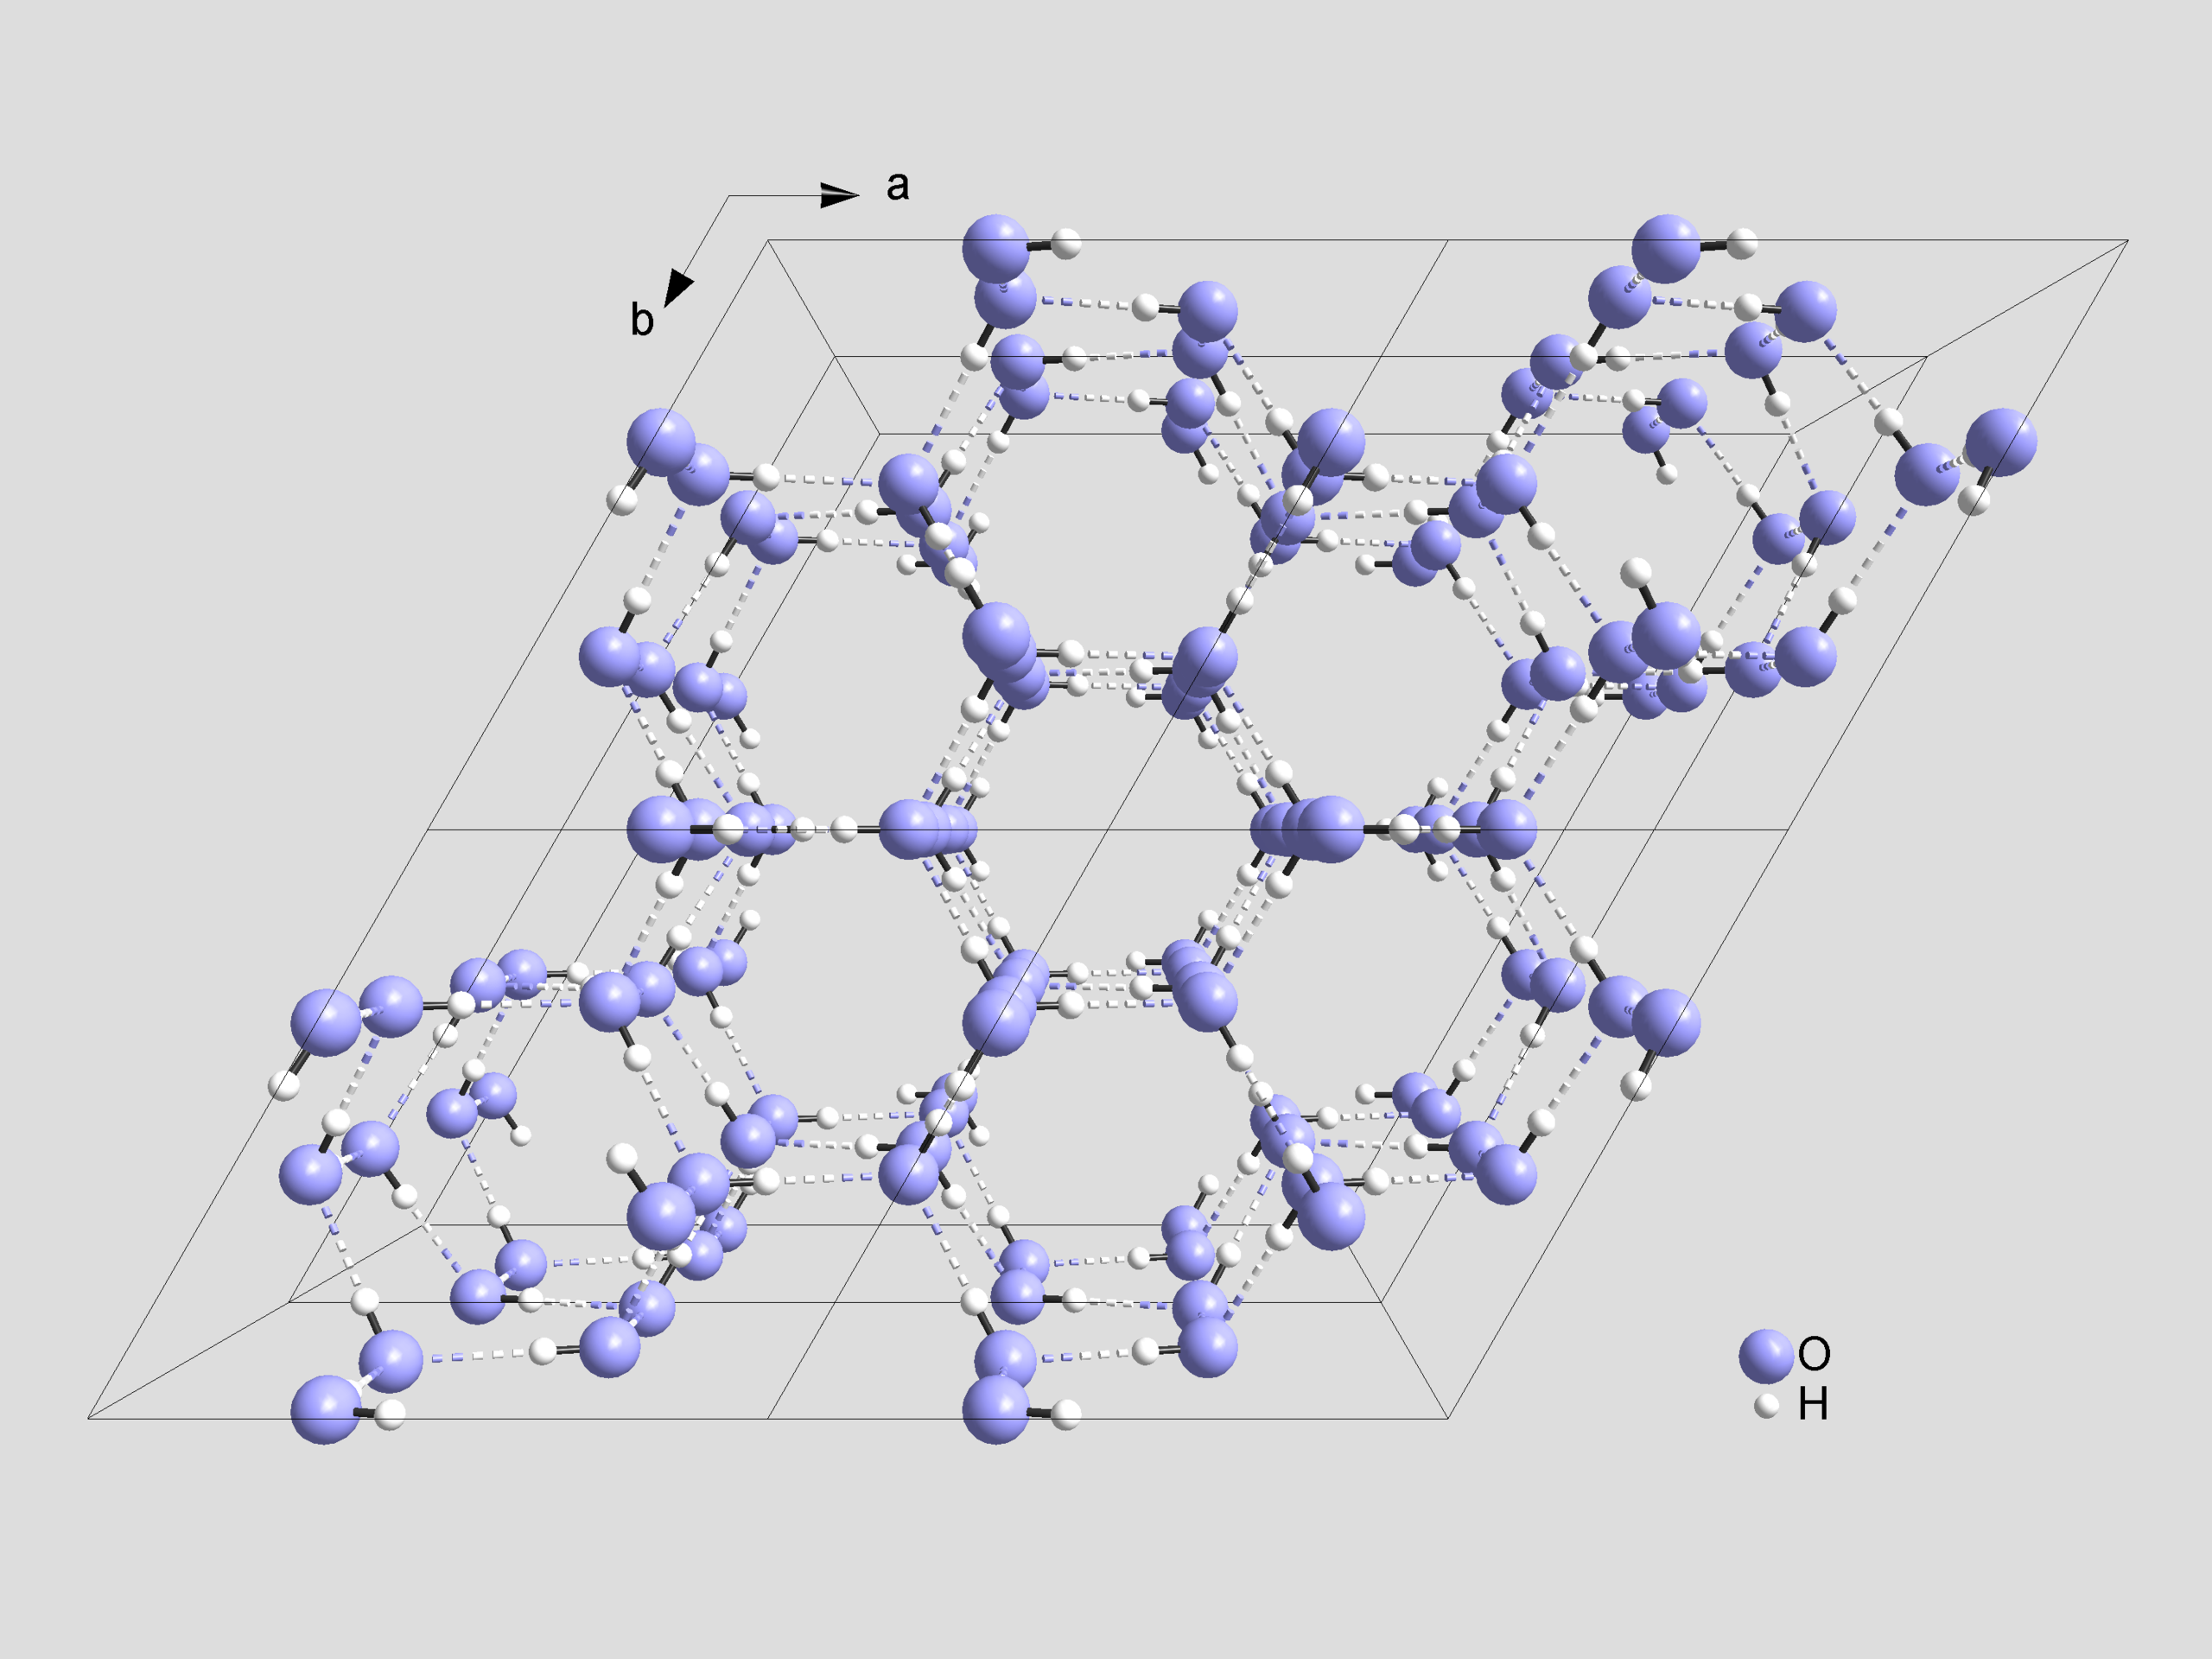
\includegraphics[width=\textwidth]{figures/Cryst_struct_ice.png}
	\captionof{figure}{\textit{The crystal structure of ice I\textsubscript{H} taken from} \cite{IceH}.}
	\label{fig:Ice}	
\end{Figure}

This large distance between oxygen atoms in the lattice means that ice is less dense than water, because the crystal structure of ice has large volumes of empty space in between the molecules; in water, the molecules aren't arranged as neatly and some molecules fill these gaps.
\section{Grotthuss Process}

The Grotthuss process refers to the phenomenon of positive electric charge moving through a body of water through the process of protons breaking away from one H\textsubscript{3}O\textsuperscript{+} ion and joining to an H\textsubscript{2}O molecule to form a new H\textsubscript{3}O\textsuperscript{+}. This process repeats, allowing the positively charged ion to migrate throughout the system.

\subsection{Historical Background}
The process was first theorised by Theodor von Grotthuss in his 1805 article \textit{M{\'e}moire sur la d{\'e}composition de l'eau et des corps qu'elle tient en dissolution {\`a} l'aide de l'{\'e}lectricit{\'e} galvanique}.\cite{Grotthuss1805}\footnote{\textit{"Memoire on the decomposition of water and of the bodies that it holds in solution by means of galvanic electricity."} It was summarised in 2005 by Samuel Cukierman \cite{Cukiermann2005} and translated into English in 2006 by R\'egis Pom\`es.\cite{Grotthuss2006} According to Bruno Jaselkis et al.,\cite{Jaselskis2007} the article had already been translated in Tillochs Philos. Mag., 1806, 25, 330-339, but I was unable to uncover a copy of this.} In this paper, he investigated the effects of a potential difference across copper and zinc electrodes immersed into a salt solution, which Grotthuss referred to as \textit{galvanic electricity}.

In the second chapter, Grotthuss attempted to explain why when this galvanic electricity was applied to water, at the positive electrode only oxygen gas was produced and at the negative electrode, only hydrogen gas. He theorised that OH molecules\footnote{It was not until 1811 that Avogadro established that water molecules are composed of two hydrogen atoms and one oxygen atom.\cite{Avogadro1811} Despite this seemingly fundamental misunderstanding of molecular water, Grotthuss still managed to come up with an accurate theory of how charge moves through it.} must feature positive and negative poles and that hydrogen and oxygen must take positive and negative states respectively. Thus, the positive electrode attracts the negative oxygen and the negative electrode attracts the positive hydrogen. Grotthuss proposed that when an oxygen atom is separated from a water molecule at the positive electrode, the remaining hydrogen attaches to a nearby water molecule, whose hydrogen detaches then reattaches to another water molecule. This process repeats until the positive charge has traveled across to the negative electrode. This process is mirrored by a process whereby, at the negative electrode, hydrogen is separated from water and oxygen jumps across the system. Grotthuss believed that by this process could be used to dissociate all the molecules in the water and separate the water into two gases.\cite{Jaselskis2007}

In the early 20\textsuperscript{th} century, efforts were made to predict and measure the ionic mobility in pure water. At the time ionic mobilities were only thought about in hydrodynamic terms, meaning that it was assumed to be due only to two factors, the applied electric field driving the mobility and the viscosity of the solution slowing the ion. Intermolecular reactions were not taken into account.\cite{Cukiermann2005, Huckel1928} Calculations of the mobilities in water using this theory did not match experimental results: the calculated mobility of H\textsubscript{3}O\textsuperscript{+} was ~6.5 times smaller than measured and the mobility for OH\textsuperscript{-}, ~3.3 times smaller. Explaining this disparity led to a return of Grotthuss' theory in the 1905 paper by V.H. Danneel.\cite{Danneel1905} Danneel identified the need for a rotation step in the process as we will discuss in section \ref{sec:mechanism}. 

\subsection{Mechanism}
\label{sec:mechanism}
The modern Grotthuss process under the influence of an electric field, as demonstrated in figure \ref{fig:GrotthussDiagram}, consists of 4 steps:


\textbf{1.} A proton approaches a water molecule which is oriented with its oxygen atom pointed towards the proton. The proton is attracted to the negatively charged oxygen atom and approaches, covalently bonding with it, forming a hydronium ion.

\textbf{2.} The hydronium ion approaches the next water molecule and shares a proton between the two molecules forming a Zundel cation.\footnote{The Zundel cation, H\textsubscript{5}O\textsubscript{2}\textsuperscript{+} is described in section \ref{sec:cations}.}

\textbf{3.} This jumping step propagates along the line of water molecules until the proton leaves the last molecule.

\textbf{4.} The molecules rotate so that they can accept another proton.
\begin{Figure}
	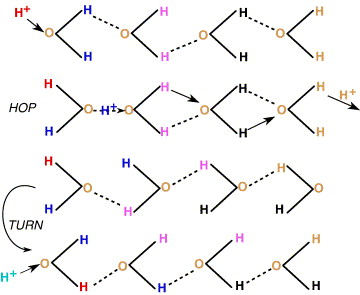
\includegraphics[width=\textwidth]{figures/ProtonHopping.jpg}
	\captionof{figure}{\textit{A simplified, 1-dimensional diagram of the modern Grotthuss mechanism showing a proton jumping from one end of the chain to the other, and the rotating of the water molecules to receive another proton. This figure was taken from} \cite{Cukiermann2005}.}
	\label{fig:GrotthussDiagram}	
\end{Figure}

Our simulation is slightly different to this specific mechanism. Instead of being driven by an external potential which causes the process to propagate in one direction, we placed the ions within a cell containing many water molecules and allowed the ions to propagate randomly.

\subsubsection{Zundel and Eigen Cations}
\label{sec:cations}
The Zundel and Eigen cations are structures formed when water molecules hydrogen bond to a hydronium ion. These structures facilitate the movement of protons from one molecule to another.

\begin{Figure}
	\includegraphics[width=\textwidth]{figures/zundel2.gif}
	\captionof{figure}{\textit{A graph showing the equilibrium solution for the position of a proton when being shared between two water molecules as part of a Zundel cation at zero temperature. The x-axis is the distance between the two oxygen atoms in angstrom and the y-axis is the difference in distance between the proton and the two oxygen atoms. The path on the graph from I to II to III, describes how the shared proton moves in a single Grotthuss jump, as shown in the pictures above the graph. This figure was taken from} \cite{Dagrada2014}.}
	\label{fig:Zundel2}	
\end{Figure}

The Zundel cation has the formula H\textsubscript{5}O\textsubscript{2}\textsuperscript{+} and is the simplest structure in which the Grotthuss process takes place, with a proton being shared between two water molecules.\cite{Zundel2006, kampschulte1970tunnel} The way the proton moves between the molecules is described in figures \ref{fig:Zundel2} and \ref{fig:Zundel}.

\begin{Figure}
	\includegraphics[width=\textwidth]{figures/zundel.gif}
	\captionof{figure}{\textit{Four graphs showing how a proton acts when being shared between two water molecules as part of a Zundel cation at two different temperatures and modelled as a classical and quantum particle. The axes are the same as for figure \ref{fig:Zundel2} and the different colours indicate the likelihood of the proton being found in each position, with purple being more likely and yellow being less likely. The red curve is the zero temperature equilibrium solution which is superimposed on the graphs as a comparison.\protect\footnotemark This figure is taken from} \cite{Mouhat2017}.}
	\label{fig:Zundel}	
\end{Figure}
\footnotetext{Note the difference between the classical and quantum simulations at 300K. In particular, note the fact that the quantum particle has a much higher probability of being equally spaced between the two molecules when the distance between the two oxygen atoms is large, whereas the classical simulation has a very low probability. This indicates that in the quantum simulation the proton is likely to tunnel between the two molecules. This is discussed further in section \ref{sec:PIMD}.}

The Eigen cation involves a proton being shared between four molecules. It has the formula H\textsubscript{9}O\textsubscript{4}\textsuperscript{+} and is made up of a hydronium ion with each of its protons hydrogen bonded to another water molecule.\footnote{In reality, water is not so neatly ordered that all the protons are always hydrogen bonded, therefore H\textsubscript{7}O\textsubscript{3}\textsuperscript{+} do also exist. Its properties are very similar to those of the Eigen cation. In addition, single protons can hydrogen bond to more than one molecule meaning that lots of different structures are possible.}
\begin{Figure}
	\includegraphics[width=\textwidth]{figures/Eigen}
	\captionof{figure}{\textit{The resonance structures of the Eigen cation. This diagram demonstrates how the positive charge can moves between the four molecules. This figure is taken from} \cite{Cations}.}
	\label{fig:Eigen}	
\end{Figure}

\section{The Tight Binding Approximation}
This section, laying out the theory of self consistent tight binding, follows the lecture notes by Paxton.\cite{Paxton2009} 

\subsection{Two Centre Approximation}
Hamiltonian matrix elements are made up of an integral of three functions: one potential\footnote{The effective potential may be written as a sum of the atom centred potentials.} and two orbitals centred at three sites. If all are on the same site, this is an \textit{on-site} matrix element. If the orbitals are on neighbouring sites\footnote{This is determined by a cut off distance.} and the potential is on one of these sites, this is a \textit{hopping} element. All other elements are neglected.

\subsection{Traditional Non Self Consistent Tight Binding Theory}
\subsubsection{Density Operator and Density Matrix} 
\label{sec:density}
The Hamiltonian in non self consistent tight binding is denoted by $H^{0}$ and is the sum of non interacting kinetic energy and the effective potential generated by some input superposition of atom centred, spherical charge densities.\cite{Finnis2003} It has a complete set of orthogonal eigenfunctions $\psi_n$ and using Dirac notation we can write,
\begin{equation}
	H^0\ket{n}=\varepsilon_n\ket{n}
\end{equation}
where $\varepsilon_n$ are the eigenvalues of $H^0$. We use this to construct the band energy,
\begin{equation}
	E_{\text{band}}=\sum_{n}f_n\varepsilon_n
\end{equation}
where $f_n$ are the occupation numbers. For an insulator the occupation numbers are: 2 if $\varepsilon_n$ is less than the Fermi energy or 0 otherwise. In a metal or molecule with a degenerate highest occupied energy level, the occupation numbers are twice the Fermi function.

The eigenstates of $H^0$ can be expanded in a \textit{linear combination of atomic(-like) orbitals} (LCAO). \cite{huheey2006inorganic}
This means that we decorate each atomic site, denoted \textbf{R}, labelling its position with respect to some origin. The orbitals have angular momentum $L = \ell m$, where $\ell$ labels the type of orbital\footnote{For water we only need to use $s$ and $p$ orbitals.} and $L$ is denoted $s$, $x$, $y$ or $z$.\footnote{This index is explained in section \ref{sec:onsite}.} The orbitals are denoted
\begin{equation}
	\ket{\textbf{R}L}=\ket{i}
\end{equation}
to simplify the orbitals and quantum numbers into a single index $i$.\footnote{$j$, $k$ and $l$ are also used.} In this way and employing Einstein's summation convention we can write
\begin{equation}
	\ket{n} = c^{n}_{i}\ket{i}
\end{equation}
where the coefficients $c^{n}_{i}$ are the eigenvectors of $H^{0}$. The parameters of the tight binding model are the matrix elements of the Hamiltonian in the LCAO basis:
\begin{equation}
	H^{0}_{ij} =\bra{i}H^{0}\ket{j}
\end{equation}
In general we can define a matrix of overlap integrals
\begin{equation}
	S_{ij}=\bra{i}\ket{j}.
\end{equation}
but for our simulations we treat the orbitals as orthogonal, thus $S_{ij} =\delta_{ij}$.
 
The time-independent Schr{\"o}dinger equation thus becomes 
\begin{equation}
	(H^{0}_{ij}-\varepsilon_{n}S_{ij})c^{n}_{i}=0
\end{equation}
which we can rearrange to work out the eigenvectors.

Next, from the eigenvectors, we want to construct a density matrix which will provide us with the band energy, local “Mulliken” charges, bond charges (in the non orthogonal case),\cite{Finnis2003} bond orders,\cite{pettifor1995bonding} interatomic forces, and in the case of time dependent tight binding, the bond currents via its imaginary part.\cite{todorov2002tight}

The density operator $\hat{\rho}$ must have the following properties \cite{Paxton2009}:

\textbf{Property 1.} Idempotency, $\hat{\rho}^2=\hat{\rho}$,

\textbf{Property 2.} $\textrm{Tr }\hat{\rho}=N$, the number of electrons,\footnote{This leads to an important property in tight binding: the Mulliken charge associated with orbital $i$ is
\begin{equation}
	\label{eq:mulliken}
	q_{i}=\sum_{n}f_{n}\sum_{j}\bar{c}^{n}_{i}S_{ij}c^{n}_{j} 
\end{equation}.}

\textbf{Property 3.} $\textrm{Tr }\hat{\rho}H^0=\sum_nf_n\varepsilon_n=E_{\text{band}}$, the band energy,

\textbf{Property 4.} $\textrm{Tr }\hat{\rho}H^0=\frac{\partial}{\partial\lambda}E_{\text{band}}$, the Hellman-Feynman theorem.

From quantum mechanics \cite{schiff2quantum,kittel1965quantum} we know that for one particle the density operator is defined as 
\begin{equation}
	\label{eq:rho}
	\hat{\rho}=\sum_{n}f_{n}\ket{n}\bra{n}.
\end{equation}
To find the density operator in the LCAO basis we define a unit operator,
\begin{equation}
	\hat{1}=\ket{i}S^{-1}_{ij}\bra{j}
	\label{eq:unit}
\end{equation}
and insert it into equation \ref{eq:rho}
\begin{equation}
	\begin{split}
		\hat{\rho}=\sum_{n}f_{n}\ket{n}\bra{n}&=\sum_{n}f_{n}\hat{1}\ket{n}\bra{n}\hat{1} \\
		&=\sum_{n}f_{n}\ket{i}c^{n}_{i}\bar{c}^{n}_{j}\bra{j}
	\end{split}
\end{equation}
and so the matrix elements of the density operator are 
\begin{equation}
	\begin{split}
		\rho_{kl}&=\sum_{n}f_{n}\bra{k}\ket{i}c^{n}_{i}\bar{c}^{n}_{j}\bra{j}\ket{l} \\
		&=\sum_{n}f_{n}S_{ki}c^{n}_{i}\bar{c}^{n}_{j}S_{jl}
	\end{split}
\end{equation}
which in an orthogonal basis is 
\begin{equation}
	\rho_{ij}=\sum_{n}f_{n}c^{n}_{i}\bar{c}^{n}_{j}
\end{equation}

\subsubsection{Density of States}
The density of states is defined as
\begin{equation}
	n(\varepsilon)=\sum_{n}\delta(\varepsilon-\varepsilon_{n})
\end{equation}
and can be used to find the band energy because of the relations
\begin{equation}
	E_{\text{band}} = \sum_{n}f_{n}\varepsilon_{n}=\sum_{n}f_{n}\int\delta(\varepsilon-\varepsilon_{n})d\varepsilon
\end{equation}

We can also define a partial density of states $n_{i}(\varepsilon)$, the density of states projected onto the orbital $i$. Using our unit operator from equation \ref{eq:unit} and the Schr\"odinger equation, we define it as
\begin{equation}
	n_{i}(\varepsilon)=\sum_{n}\sum_{j}\bar{c}^{n}_{i}S_{ij}c^{n}_{j}\delta(\varepsilon-\varepsilon_n).
\end{equation}
Here, $j$ is summed over explicitly and $i$ is not summed over.

\subsubsection{Tight Binding Bond Model}
\label{sec:TBBM}

In the traditional tight binding approximation we have
\begin{equation}
	E_{\text{tot}}=E_{\text{band}}+E_{\text{pair}}
\end{equation}
for the total energy in the band model, where $E_{\text{pair}}$ is a repulsive energy between each pair of atoms. To derive the \textit{covalent bond energy} \cite{sutton1993electronic,Sutton_1988} we remove the diagonal elements of $E_{\text{band}}$: 
\begin{equation}
	\begin{split}
		E_{\text{bond}}&=\frac{1}{2}\sum\limits_{\substack{ij \\ \textbf{R'}\neq\textbf{R}}}2\rho_{ij}H^0_{ji} \\
		&=\frac{1}{2}\sum\limits_{\substack{\textbf{R}L\textbf{R'}L' \\ \textbf{R'}\neq\textbf{R}}}2\rho_{\textbf{R}L\textbf{R'}L'}H^0_{\textbf{R}L\textbf{R'}L'}.
	\end{split}
\end{equation}
The remaining terms are grouped with the corresponding energies in the free atom. In non self consistent tight binding, on site elements of $H^{0}$ are simply the eigenvalues of the Hamiltonian:
\begin{equation}
	H^{0}_{\textbf{R}L\textbf{R}L'}=\varepsilon_{\textbf{R}\ell}\delta_{LL'}.
\end{equation}
These are $\varepsilon_{s}$ and $\varepsilon_{p}$, two of the parameters of the tight binding model referred to in table \ref{tab:H2Otable}. 

In addition we assume certain orbital occupancies in the free atom, which we label $N_{\textbf{R}\ell}$, but after diagonalisation of the Hamiltonian we find that these orbitals have occupancies given by the diagonal elements of the density matrix. Therefore there is a change in energy in the transition between the free atom limit to condensed matter which is the promotion energy: 
\begin{equation}
\label{eq:prom}
	\begin{split}
		E_{\text{prom}}&=\sum_{\textbf{R}L}(\rho_{\textbf{R}L\textbf{R}L}H^{0}_{\textbf{R}L\textbf{R}L}-N_{\textbf{R}\ell}\varepsilon_{\textbf{R}\ell} )\\
		&=\sum_{\textbf{R}L}(\rho_{\textbf{R}L\textbf{R}L}-N_{\textbf{R}\ell})
	\end{split}
\end{equation}

Thus the \textit{binding energy} is the total energy minus the energy of the free atoms,
\begin{equation}
	E_{\text{B}}=E_{\text{bond}}+E_{\text{prom}}+E_{\text{pair}}.
\end{equation}
The force between a pair of atoms is $-\nabla E_{\text{pair}}$ for that particular pair, minus $\text{Tr}\nabla H^{0}$, assuming that the on-site elements stay constant; this makes the fully non self consistent tight binding approximation.

\subsection{Self-consistent Tight Binding}
\label{sec:Self_consistent}

The local charge neutrality of the tight binding bond model is insufficient to describe systems where a large part of the total energy is due to electrostatic attraction, like hydrogen bonding in water. A way to deal with this is to treat the total charge transfer at each site $\Delta q_{\text{R}}$ from equations \ref{eq:mulliken} and \ref{eq:prom} as a point charge.\cite{hafner2013structures,majewski1986crystal}. The Hamiltonian is written
\begin{equation}
	H=H^{0}+H'
\end{equation}
with $H'$ made up of two terms: the Madelung energy of the lattice of point charges \cite{Madelung1919} and a positive energy, $U_{\textbf{R}}\Delta q_{\text{R}}^{2}$ where $U_{\textbf{R}}$ is the \textit{Hubbard U}.\cite{Hubbard1963} An extension to this allows the charge to be expressed as multipoles instead of just monopoles.\cite{Finnis1998,schelling1998self}

From density functional theory, we can expand the Hohenber-Kohn total energy \cite{Kohn1964} about some reference energy $\rho^{0}(\textbf{r})$ \cite{elstner1998self} to get 
\begin{equation}
	\begin{split}
		E^{(2)}&=\sum_{n}f_{n}\bra{n}H^{0}\ket{n} \\
		&-\int \rho^{0} (\textbf{r}) V^{0}_{xc} (\textbf{r}) d\textbf{r} - E^{0}_{\text{H}} + E^{0}_{\text{xc}} +E_{\text{ZZ}} \\
		&+\frac{1}{2}\int d\textbf{r}\int d\textbf{r}'\bigg \{e^{2}\frac{\delta\rho(\textbf{r})\delta\rho(\textbf{r}')}{|\textbf{r}-\textbf{r}'|} \\
		& +\delta\rho(\textbf{r})\frac{\delta^{2}E_{\text{xc}}}{\delta\rho(\textbf{r}\delta\rho(\textbf{r}')}\delta\rho(\textbf{r}'\bigg\}
	\end{split}
\end{equation} 
where $E^{0}_{H}$ is the Hartree energy\footnote{The Hartree energy is defined as $E^{0}_{H}=\hbar^{2}/m_{e}a^{2}_{0}$.} and $E^{0}_{\text{xc}}$ and $V^{0}_{\text{xc}}$ are the exchange-correlation energy and potential belonging to the reference density. Lines one and two make up the Harris-Foulkes first order functional;\cite{Harris1985} the first term is the band energy and the second term is the interaction term plus the ion-ion pair potential, $E_{ZZ}$. In self consistent tight binding the last two lines are approximated by a generalised Madelung energy \cite{Madelung1919} and a Hubbard energy,\cite{Hubbard1963} which adds a second order energy to the binding energy:
\begin{equation}
\label{eq:Electrostatic}
	E_{2}=\frac{1}{2}e^{2}\sum_{\textbf{R}L\textbf{R}'L'}Q_{\textbf{R}'L'}+\frac{1}{2}\sum_{\textbf{R}}U_{\textbf{R}}\Delta q^{2}_{\textbf{R}}.
\end{equation}
The first term is a classical interaction between multipoles and the second term is as above. $\tilde{B}_{\textbf{R}'L'\textbf{R}L}$ is the Madelung matrix.

$Q_{\textbf{R}L}$ is the multipole moment at site \textbf{R} with angular momentum $L$, constructed from the eigenvectors of the Hamiltonian:
\begin{equation}
	\label{eq:multipole}
	Q_{\textbf{R}L}=\sum_{L'L''}\sum_{n}f_{n}\bar{c}^{n}_{\textbf{R}L'}c^{n}_{\textbf{R}L''}\bigg \langle\textbf{R}L'\bigg | \hat{Q}_{\textbf{R}L}\bigg |\textbf{R}L''\bigg \rangle
\end{equation}
in which the multipole moment operator is \cite{stone2013theory}
\begin{equation}
	\hat{Q}_{\textbf{R}L}=\hat{r}^{\ell}Y_{L}(\hat{\textbf{r}})
\end{equation}
with $Y_{L}(\hat{\textbf{r}})$ being the standard spherical harmonic. Expanding out the matrix element of $\hat{Q}_{\textbf{R}L}$ we get
\begin{equation}
	\label{eq:Delta}
	\begin{split}
		 \bigg \langle \textbf{R}L' \bigg | {\hat{Q}}_{\textbf{R}L} \bigg | \textbf{R}L'' \bigg \rangle &=\int r^{2}\text{d}r\,f_{R\ell'}f_{R\ell''}r^{\ell}\\&\,\,\,\,\,\,\iint \text{d}\Omega \,Y_{L''}Y_{L'}Y_{L} \\
		&=\Delta_{\ell'\ell''\ell}C_{L'L''L},
	\end{split}
\end{equation} 
from which we get the tight binding parameters $\Delta_{\ell'\ell''\ell}$.

By expanding the electrostatic potential from equation \ref{eq:Electrostatic} in the neighbourhood of \textbf{R} into spherical waves, we can write
\begin{equation}
	V_{\textbf{R}}(\textbf{r})=\sum_L V_{\textbf{R}L}r^{\ell}Y_{L}(\textbf{r})
\end{equation}
and the $\textbf{R}L$ coefficient is 
\begin{equation}
	V_{\textbf{R}L}=\sum_{\textbf{R}'L'}\tilde{B}_{\textbf{R}L\textbf{R}'L'}.
\end{equation}
Using the same method as in equation \ref{eq:multipole} we can find the matrix elements of $H'$ which are 
\begin{equation}
	H'_{\textbf{R}L'\textbf{R}L''}=U_{\textbf{R}}\Delta q_{\textbf{R}}\delta_{L'L''}+e^{2}\sum_L V_{\textbf{R}L}\Delta_{\ell'\ell''\ell}C_{L'L''L}
\end{equation}
where $C_{L'L''L}$ are the Gaunt coefficients, given by the integral
\begin{equation}
	C_{L'L''L} = \iint d\Omega Y_{L''}Y_{L'}Y_{l}
\end{equation}

Now we have all the terms we need for self consistent tight binding. The method is described in section \ref{sec:self-consistent}.

Finally, the interatomic force on an atom at site \textbf{R} can be found to be 
\begin{equation}
	\textbf{F}^{\text{es}}_{\textbf{R}}= -\sum_L Q_{\textbf{R}L}\nabla V_{\textbf{R}L}
\end{equation}
\subsection{Tight Binding in Water}
\label{sec:tbe_water}

\begin{minipage}{\linewidth}
	\begin{center}
		\scriptsize
		\captionof{table}{\textit{A complete list of the parameters used in the tight binding model taken from reference} \cite{Lozovoi2014}. \textit{All quantities are in Rydberg atomic units.}}
		\label{tab:H2Otable}
		\begin{tabularx}{\linewidth}{XYY}
			\hline \hline
   			\multicolumn{3}{c}{On-site parameters} \\
   			\hline
  			& O & H \\
  			\hline
			$\varepsilon_s$ & $-2.1164$ & $-1$ \\
			$\varepsilon_p$ & $-1.1492$ & \\
			Hubbard $U$ & $1.0775$ &  $1$ \\
			$\Delta_{spp}$ & $-0.9430$ & \\
			$\Delta_{ppd}$ & $0$ & \\
			\multicolumn{3}{c}{Bond integrals, $V_{\ell'm^,}$ and scaling} \\
			\hline
			& O$-$H & O$-$O \\
			Function & GSP & GSP \\
			\hline
			$V^0_{ss\sigma}$ & $-0.5018$ & $-0.0150$ \\
			$V^0_{sp\sigma}$ && $0.0020$ \\
			$V^0_{ps\sigma}$ & $-0.4362$ & $-0.0020$ \\
			$V^0_{pp\sigma}$ && $0.0500$ \\
			$V^0_{pp\pi}$ && $-0.0200$ \\
			$n_{ss\sigma}$ & $2.0963$ & $2$ \\
			$n_{sp\sigma}$ && $2$ \\
			$n_{ps\sigma}$ & $1.5019$ & $2$ \\
			$n_{pp\sigma}$ & & $3$ \\
			$n_{pp\pi}$ && $3$ \\
			$n_c$ & $4.0561$ & $6$ \\
			$r_0$ & $1.8094$ & $5.6$ \\
			$r_c$ & $3.7985$ & $9.0$ \\
			\multicolumn{3}{c}{Pair potentials, $\phi$ and scaling} \\
			\hline
			& O$-$H & O$-$O \\
			Function & GSP & EPL \\
			\hline
			$\phi^0$ & $0.73669$ & \\
			$n_c$ & $6.3096$ & \\
			$r_0$ & $1.8094$ & 5.6 \\
			$r_c$ & $3.3550$ & \\
			$\phi^0_1$ && $4.0306\times 10^{-3}$ \\
			$\phi^0_2$ && $-2.0265\times 10^{-3}$ \\
			$m_1$ && 10 \\
			$m_2$ && 6 \\
			$p_1$ && 0 \\
			$p_2$ && 0 \\
			\multicolumn{3}{c}{Cut-off distances [$r^{(1)}_{\text{cut}}$, $r^{(2)}_{\text{cut}}$]} \\
			\hline
			& O$-$H & O$-$O \\
			\hline
			$r^{(1)}_{\text{cut}}$ & $2.1$ & $8$ \\
			$r^{(2)}_{\text{cut}}$ & $5.5$ & $11$ \\
			\hline \hline \\	    
		\end{tabularx}
	\end{center}
\end{minipage}
In addition to these, there is a short range repulsive H-H pair potential. There are no other bonded interactions between hydrogen atoms in our model since these are considered insignificant. The weak repulsion is added with the sole purpose of avoiding polarization catastrophes where two H atoms that happen to be close enough during a simulation, might spontaneously pick up opposite charges and be pulled towards each other.

\subsubsection{On Site Terms}
\label{sec:onsite}
The on site matrix elements of the non self consistent Hamiltonian as defined in section \ref{sec:TBBM} are 
\begin{equation}
	H^{0}_{\textbf{R}L,\textbf{R}L'}=\varepsilon_{\textbf{R}\ell}\delta_{\ell\ell'}.
\end{equation}
$L$ is as defined in section \ref{sec:density}.

Additionally, we have the self consistency terms, $\Delta$ and the Hubbard $U$, which are used in the method described in section \ref{sec:self-consistent}.
\subsubsection{Bond Integrals}
\begin{Figure}
	\centering
	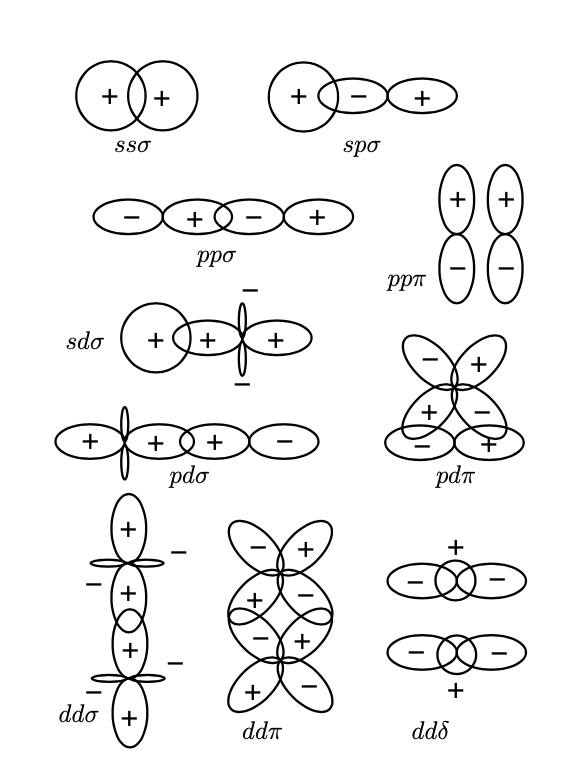
\includegraphics[width=0.8\textwidth]{figures/bond_integrals.png}
	\captionof{figure}{\textit{The fundamental bond integrals between $s$, $p$ and $d$ orbitals. These bond integrals are used to assemble the total bond integral between orbitals at any distance and orientation via the Slater-Koster table \cite{Slater1954} This figure is taken from \cite{Paxton2009}}}
	\label{fig:Bond Integrals}
\end{Figure}
\noindent The hopping elements of the non self consistent Hamiltonian between two atoms in positions \textbf{R} and \textbf{R}' are 
\begin{equation}
	H^{0}_{\textbf{R}L,\textbf{R}'L'}=E_{LL'}(\textbf{R}-\textbf{R}')
\end{equation}
where $\textbf{R}\neq\textbf{R}'$.\cite{Lozovoi2014}

These values are calculated with the Slater-Koster table (see table \ref{tab:Slater-Koster}), using the parameters in table \ref{tab:H2Otable} and the Goodwin-Skinner-Pettifor scaling set out in section \ref{sec:scaling}.

\begin{center}
	\captionof{table}{\textit{The Slater-Koster table of interatomic matrix elements as functions of the direction cosines of the vector from the left state to the right state for \textit{s} and \textit{p} orbitals. The potentials refer to the different ways orbitals can interact shown in figure \ref{fig:Bond Integrals}. This table was taken from }\cite{Slater1954}.}
	\label{tab:Slater-Koster}
	\begin{tabularx}{\linewidth}{XX}
		\hline
		$E_{\text{s, s}} =$ & $V_{ss\sigma} $ \\
		$E_{\text{s, x}} =$ & $lV_{sp\sigma} $ \\
		$E_{\text{x, x}} =$ & $l^{2}V_{pp\sigma} +(1-l^{2})V_{pp\pi}$ \\
		$E_{\text{x, y}} =$ & $lmV_{pp\sigma} + lmV_{pp\pi}$ \\
		$E_{\text{x, z}} =$ & $lnV_{pp\sigma} + lnV_{pp\pi}$ \\
		\hline 
	\end{tabularx}
\end{center}

\subsubsection{Pair Potentials}
The energy due to the potential between each pair of atoms is given by:
\begin{equation}
	E_{\text{pair}}=\frac{1}{2}\sum_{\textbf{R} \neq \textbf{R}'}\phi_{\textbf{RR}'}(|\textbf{R}-\textbf{R}'|)
\end{equation}
where \textbf{R} and \textbf{R}$'$ are two atomic sites and $\phi_{\textbf{R}\textbf{R}'}$ is calculated using the values given in table \ref{tab:H2Otable} according to the scaling laws discussed in section \ref{sec:scaling}.\cite{Sheppard2014}

\subsubsection{Scaling}
\label{sec:scaling}
The scaling laws in the above table are Goodwin-Skinner-Pettifor (GSP) scaling,\cite{Goodwin1989} which has the form,
\begin{equation}
	f(r)=A(r_{0}/r)^{n}\exp{n[-(r/r_{c})^{n_{c}}+(r_{0}/r_{c})^{n_{c}}]}
\end{equation}
and exponential $\times$ power law (EPL) scaling,\cite{Lozovoi2014} which has the form
\begin{equation}
	f(r)=\sum_i A_{i}(r_{0}/r)^{m_{i}}\exp[-p_{i}(r-r_{0})]
\end{equation}
where A denotes the $V^0$ and $\phi_{0}$ values. This scaling is used because the O-O pair potential is repulsive at short distances but attractive at long range. The other values are all taken from table \ref{tab:H2Otable}.

\subsection{Other Simulation Methods}

Tight binding is one of a number of electronic structure methods used to simulate water. Simulations of the Grotthuss process in bulk water have been constructed by Han et al. \cite{Han2005} and most recently by White et al. \cite{White2017}, both using \textit{ab initio} computational chemistry methods. Small scale simulations have also been performed \cite{samala2018protonated, chen2018hydroxide} using density functional theory.\cite{Gillan2016}

The Zundel cation has been simulated using variational quantum Monte Carlo and path integral Langevin dynamics.\cite{Mouhat2017} This is a particularly interesting simulation to us as it uses a very similar method to the one we want to use in section \ref{sec:PIMD}.

\section{Methods}
\label{sec:method}

\subsection{Empirical Tight Binding}
Having created our tight binding model, the next stage was to create simulations in the empirical tight binding (TBE) code where the Grotthuss process could be observed and measured. For our the simulations, we used TBE in three main ways:

\subsubsection{Self-consistency}
\label{sec:self-consistent}
The tight binding code uses the method described in reference \cite{Paxton2009}. The steps are,
\begin{enumerate}
	\item Solve the eigenproblem for $H^{0}$, the non self consistent Hamiltonian, finding the eigenvector expansion coefficients.
	\item Build the multipole moments and find the components, $V_{\textbf{R}L}$, of the potential.
	\item Assemble the elements of $H'$.
	\item Solve the eigenproblem for $H=H^{0}+H'$.
	\item Repeat until self consistent. The conditions for this criterion are defined in section \ref{sec:ITER}.
\end{enumerate}

\subsubsection{Molecular Statics}
\label{sec:relax}
We used molecular statics to relax our configurations to the point where the forces were small enough that the atoms would be stable in molecular dynamics simulations. We used two of the relaxations modes, the Fletcher-Powell algorithm\footnote{This algorithm works by finding the minumum along a line, changing line and then updating the Hessian matrix.}\cite{Fletcher1980,Davidson1959,CTRL} and the Broyden algorithm.\footnote{This method is essentially a Newton-Raphson algorithm with the Hessian matrix and direction of descent being updated after each step.}\cite{Broyden1965}

We set the XTOL and GTOL tolerances \cite{CTRL} to $10^{-5}$, the number of iterations (NIT) to $10000$ and the distance step (STEP) to between $0.1$ and $0.001$ (using a large step for configurations which relaxed easily, and reducing it where necessary).

\subsubsection{Molecular Dynamics}
\label{sec:MD}
TBE performs molecular dynamics using the method set out in source \cite{martyna1996explicit}, i.e. using reversible integrators which employ Liouville operators.

For all our simulations we ran molecular dynamics for a maximum of 10ps with 0.5fs between time steps. We used the NVT mode (conserved number of particles, volume and temperature) since it is the most stable. The xyz and md files\footnote{These files are explained in section \ref{sec:analysis}.} were written to in every frame.

\subsection{Using Empirical Tight Binding Code}
\label{sec:TBE}
Empirical tight binding is included as part of the Questaal Suite of electronic structure programs. It provides charge and spin self consistency, and molecular statics and dynamics. All the programs in the suite use the same basic input file containing all the variables that can be changed. It is referred to as the CTRL file \cite{CTRL} and is broken up into categories \cite{TBE} that can be either be written directly into the CTRL file or read from a separate file using the command \texttt{\% include}.\footnote{Below I have written a summary of just the categories, variables and command line switches used in the project. A complete list can be found in source \cite{CTRL} and the other pages on the Questaal website.}

\subsubsection{STRUC Category} The STRUC category defines the simulation cell and number of atoms and species in it.
\begin{itemize}
	\item{\textbf{NBAS} The number of atoms in the simulation.}
	\item{\textbf{NSPEC} The number of species of atoms in the simulation.}
	\item{\textbf{PLAT} Three dimensionless 3-vectors defining the simulation cell.}
	\item{\textbf{ALAT} A scaling, in atomic units, of the lattice and basis vectors.}
\end{itemize}

\subsubsection{SPEC Category} The SPEC category defines a number of values for each species of atom.
\begin{itemize}
	\item{\textbf{ATOM} The species of the atom.}
	\item{\textbf{Z} The nuclear charge.}
	\item{\textbf{AMASS} The nuclear mass in a.u.}
	\item{\textbf{QPOL} Up to ten $\Delta_{\ell'\ell''\ell}$ parameters.\footnote{See section \ref{sec:Self_consistent}}}
\end{itemize}
\subsubsection{POS Category} The POS category specifies the atoms in the cell and whether or not they can be relaxed using molecular statics. Each atom has the following values:
\begin{itemize}
	\item{\textbf{ATOM} The species of the atom; it must be one of the ones specified in the SPEC category.}
	\item{\textbf{POS} The x, y and z positions. These must be within the cell defined in the STRUC category.}
	\item{\textbf{RELAX} This specifies whether the atom can be relaxed in the x, y and z directions.}
\end{itemize}
\subsubsection{DYN Category}
\label{sec:DYN}
The DYN category contains all the variables needed to run molecular static relaxation and molecular dynamics.
\begin{itemize}
	\item \textbf{MD} Specifies molecular dynamics.
	\begin{itemize}
		\item\textbf{MODE} Specifies NVE, NVT or NPT molecular dynamics.\footnote{These are the quantities that the MD simulation tries to keep constant: N, V, P, T and E are number of particles, volume, pressure, temperature, and energy respectively.}
		\item\textbf{TSTEP} Time between MD steps. 
		\item\textbf{TEMP} Temperature of simulation.
		\item\textbf{TIME} Total time of MD simulation.
		\item\textbf{P} Pressure of simulation.
	\end{itemize}
	\item \textbf{MSTAT} Specifies molecular statics.
	\begin{itemize}
		\item\textbf{MODE} Specifies the molecular statics mode.
		\item\textbf{HESS} If true, reads the Hessian matrix\footnote{A Hessian matrix is a $3 \times 3$ matrix used in molecular statics made up of second order partial derivatives of the form $H_{ij}= \partial^{2}E/\partial x_{i}\partial x_{j}$.} from file if possible. 
		\item\textbf{XTOL} Convergence criterion for change in atomic displacements.
		\item\textbf{GTOL} Convergence criterion for tolerance in forces.
		\item\textbf{STEP} Initial (and maximum) step length.
		\item\textbf{NIT} Maximum relaxation iterations.
		\item\textbf{NKILL} Number of iterations after which Hessian should be removed.
	\end{itemize}
\end{itemize}
\subsubsection{ME Category} The ME category tells the program what Hamiltonian matrix
      to use and defines how the bond integrals and pair potentials decay and cut off.
\begin{itemize}
	\item The category starts with an integer which specifies the mode to define the matrix elements.
	\item Next, a pair of species are specified. We have to define the interactions between all the species we use, and we also have to specify pairs in both order ie, O H and H O.
	\item \textbf{MEMODE} This allows each species pair to have a different mode.
	\item \textbf{PPMODE} The pair potential mode.
	\item The code creates a cut off polynomial which smoothly cuts off pair potentials and bond integrals. It has the inputs:
	\begin{itemize}
	    \item \textbf{POLY} The degree of the cut off polynomial.
	    \item \textbf{CUTMOD} The cut off mode.
		\item \textbf{CUTPP} The cut off radii $r_{1}$ and $r_{2}$. The cut-off polynomial is defined so as to match value and slope at $r_1$ and to have zero value and slope at $r_2$.
	\end{itemize}
	\item These are followed by a $\vert$ which specifies that we are defining the rules for the Hamiltonian. This is followed by the matrix elements. We only used MEMODE = 5, the Goodwin-Skinner-Pettifore mode which was defined in section \ref{sec:tbe_water}. In this mode each matrix element requires 5 numbers, read in the order $V$, $n$, $n_{c}$, $r_{0}$, $r$. The matrix elements are each written on their own line in the order $V_{ss\sigma}$, $V_{sp\sigma}$, $V_{pp\sigma}$, $V_{pp\pi}$.
	\item \textbf{CUT} We then have to enter the cut off radii, as defined above, for each matrix element.	
\end{itemize}
\subsubsection{START Category} The START category is used to read on-site matrix elements.
\begin{itemize}
	\item{\textbf{ATOM} Specifies the species of the atom.}
	\item{\textbf{Q} Three numbers for each subshell specifying the number of electrons, the on-site Hamiltonian elements $\varepsilon$ and the Hubbard U for each class}
\end{itemize}
\subsubsection{TB Category} The TB category defines most of the species independent, TBE specific inputs.
\begin{itemize}
	\item \textbf{MOL} Turns on molecular mode which means that there are no periodic boundar conditions and the total charge of the system doesn't have to be zero.
	\item \textbf{RMAXH} The Hamiltonian cut-off length.
	\item \textbf{FORCES} Tells the code to calculate forces.
	\item \textbf{RHO} Tells the code to calculate the local projection of charges.
\end{itemize}
\subsubsection{BZ Category} Category BZ holds information concerning the numerical integration of quantities such as energy bands over the Brillouin Zone.
\begin{itemize}
	\item \textbf{METAL} If set to true the code calculates the energy bands and their weights in two band passes, otherwise they are set in advance, treating the cell as an insulator.
	\item \textbf{W} Setting this to large values broadens the sampling width for Gaussian sampling integration.
	\item \textbf{ZVAL} Manually specifies the number of electrons to accumulate.
\end{itemize}
\subsubsection{ITER Category}
\label{sec:ITER} 
The ITER category contains the information needed to perform self-consistency iterations.
\begin{itemize}
	\item{\textbf{CONV} Maximum energy change between steps for self-consistency to be reached.}
	\item{\textbf{CONVC} The maximum RMS difference between the densities n\textsuperscript{out} and n\textsuperscript{in}.}
	\item{\textbf{NIT} The maximum number of iterations to reach self-consistency.}
	\item\textbf{MIX} The rules for mixing input and output density when reaching self-consistency.
	\begin{itemize}
		\item \textbf{An} specifies the maximum number of prior iterations to include in the mixing.
		\item \textbf{k} specifies the number of iterations after which the program kills mixing.
	\end{itemize}
\end{itemize}
\subsubsection{Command Line Switches}
Command line switches are specified after the \texttt{tbe} command using \texttt{--SWITCH}, changing the word switch for our switch. Additionally, we can change any variable from the command line using \texttt{-vVARIABLE=} changing the word variable for the variable we want to alter.
\begin{itemize}
	\item \textbf{pr} Specifies the verbosity of the output file.
	\item \textbf{st} Starts a new molecular dynamics run.
	\item \textbf{rpos} Reads positions from an external file.
	\item \textbf{wpos} Writes positions to an external file.
	\item \textbf{md} Writes MD information to the MD file every n steps.
	\item \textbf{xyz} Writes to the xyz file every n steps.
\end{itemize}

\subsection{Hydronium and Water Cells}
\subsubsection{Creating H\textsubscript{3}O\textsuperscript{+}}
\label{sec:making_h3o+}
To run simulations of the Grotthuss process, I had to be able to insert a hydronium ion into various ensembles of water without disrupting the ensemble such that it became unstable. To do this I wrote a script whereby I inserted the coordinates of the molecule I wanted to replace and calculated the vectors from the oxygen to each of the hydrogens, $\bf{v}_1$ and $\bf{v}_2$. The script then took a normalised cross product of $\bf{v}_1$ and $\bf{v}_2$ to create a third vector, $\hat{\bf{v}}_3$ which was normal to the plane on which the three atoms lay. A fourth vector, $\bf{v}_4$, would then be created by rotating $\bf{v}_1$ about $\hat{\bf{v}}_3$ by \ang{113.6} \footnote{This is the approximate H-O-H bond angle in a hydronium ion.\cite{Tang1999}} using the rotation matrix $R(\boldsymbol{\hat{\textbf{n}}},\theta)$.\footnote{The rotation matrix about an arbitrary unit vector $\boldsymbol{\hat{\textbf{n}}}$ is defined: 
\begin{equation}
	R(\boldsymbol{\hat{\textbf{n}}},\theta)=\begin{pmatrix}
	\cos{\theta}+n_1^2(1-\cos{\theta}) & 
	n_1n_2(1-\cos{\theta})-n_3\sin{\theta} & 
	n_1n_3(1-\cos{\theta})+n_2\sin{\theta}) \\
	n_1n_2(1-\cos{\theta})+n_3\sin{\theta} & 
	\cos{\theta}+n_2^2(1-\cos{\theta}) & 
	n_2n_3(1-\cos{\theta})-n_1\sin{\theta}) \\
	n_1n_3(1-\cos{\theta})-n_2\sin{\theta} & 
	n_2n_3(1-\cos{\theta})+n_1\sin{\theta} & 
	\cos{\theta}+n_3^2(1-\cos{\theta})
	\end{pmatrix}
\end{equation}
where $n_1$, $n_2$ and $n_3$ are the components of the unit vector being rotated about, $\boldsymbol{\hat{\textbf{n}}}$, and $\theta$ is the angle of rotation.} An Oxygen atom is placed at $\bf{r}$ and hydrogen atoms are placed at $\bf{r} + \bf{v}_1$ and $\bf{r} + \bf{v}_4$.

To determine the position of the third hydrogen atom, we used the positions of the other three atoms to estimate its position, then the script checked each position within a range $10$ Bohr in the x, y and z directions at intervals of $0.05$ Bohr. The script calculated the $\text{H}-\text{O}-\text{H}$ bond angle between the new position and each of the other hydrogen atoms, $\theta_1$ and $\theta_2$, and checked whether they were within 0.05 radians of the bond angle taken from the literature, $\theta_0$.\cite{Tang1999} It performed a least squares regression on all the points passing this criterion by calculating a value x using the formula,
\begin{equation}
	x = (l - l_{0}) ^ 2 + (\theta_1 - \theta_0) ^ 2 +(\theta_2 - \theta_0) ^ 2
\end{equation}
where $l$ is the distance between the new position and the oxygen atom and $l_0$ is the goal bond length: the length of the vector $\bf{v}_1$. The script choose the position with the smallest value of $x$ and then performed again at all points within $0.1$ Bohr at intervals of $0.001$ Bohr and then again two more times each with intervals 100 times smaller. This gives a final position correct to within $10^{-7}$ Bohr. 

\subsubsection{Elongated Cuboid}
\label{sec:longbox}

\begin{Figure}
	\centering
	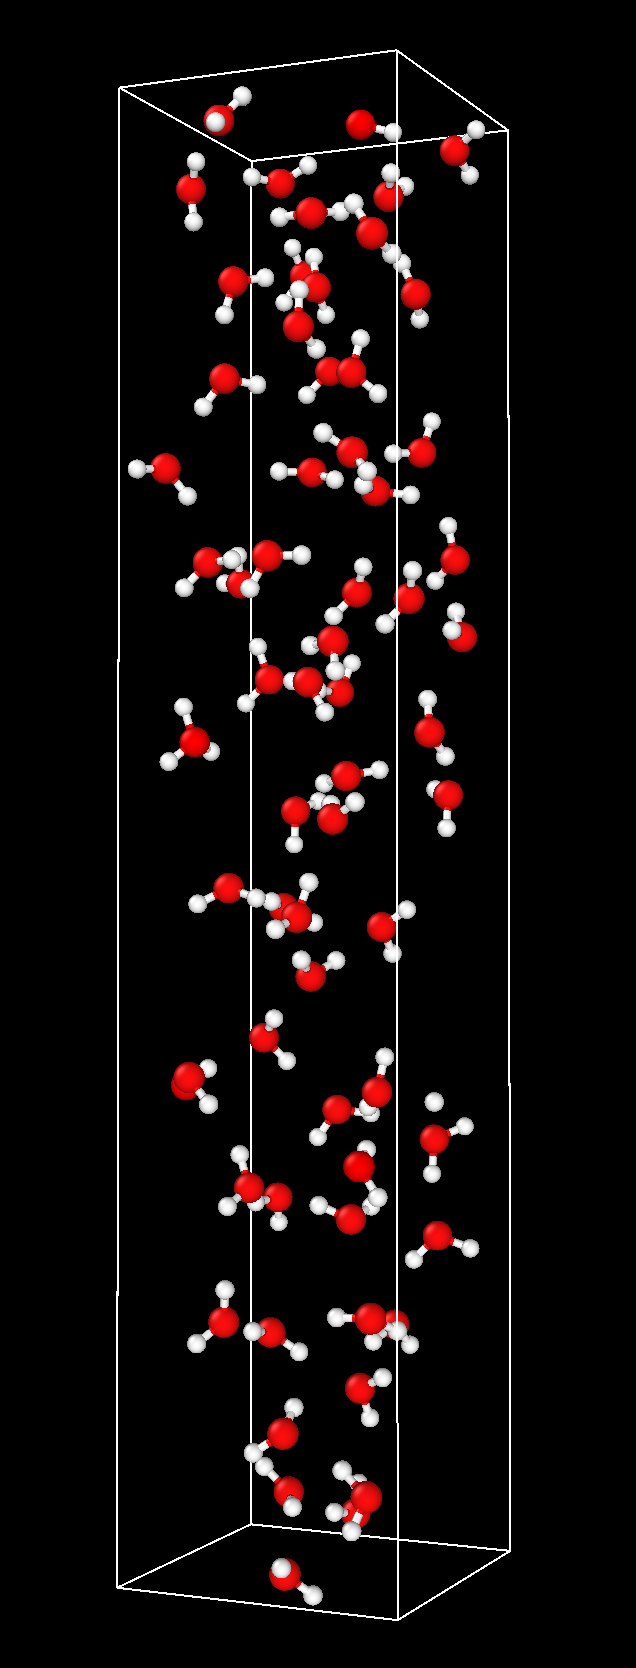
\includegraphics[width=0.6\textwidth]{figures/64}
	\captionof{figure}{\textit{The cell containing 62 water molecules, a hydronium ion and a hydroxide ion, arranged in an elongated cuboid. Oxygen atoms are coloured red and hydrogen atoms are coloured white.}}
	\label{fig:LongBox}	
\end{Figure}
The first plan for a bulk calculation of the Grotthuss process was to create an elongated cuboid cell with a number of water molecules, a hydronium ion at the centre and a hydroxide ion near one of the corners. We were worried that a small cube might have ions would be too close together to allow for detailed molecular dynamics, since they could quickly meet and turn into two water molecules, and a large cube would have too many atoms to reasonably simulate. Having the ions further apart would give us a better chance of seeing the hydronium to water proton jumping.

I created this cell from a much larger spherical water cell,\cite{WaterXYZ} by first placing the cuboid in the centre of the sphere and deleting all the atoms that didn't lie within the box. I then wrote a script that deleted all the atoms where part of their molecule had been deleted: it checked that each oxygen atom had two hydrogen atoms within 1.1 water bond lengths, and that each hydrogen had one oxygen atom within 1.1 water bond lengths. Any atom failing these tests was deleted, leaving 64 water molecules.

Next, to correct the density, we calculated the density of the box and multiplied the lengths of the sides of the box and the position vectors of the oxygen atoms by $\sqrt[3]{\frac{\rho}{\rho_{water}}}$. To preserve the bond lengths in the water molecules, the positions of the hydrogen atoms were not scaled in the same way. Instead, we found the vector of the displacement of the oxygen atom in its water molecule and added that vector to the position of the atom.

After this, we tried to relax the positions of the water molecules using molecular statics with 100 steps of 0.01 and 200 self consistency iterations at each step. However, at the end of this process the rms difference only reduced to ~0.01, too high to use in molecular dynamics.

\subsubsection{Ring}
\label{sec:ring}
\begin{Figure}
	\centering
	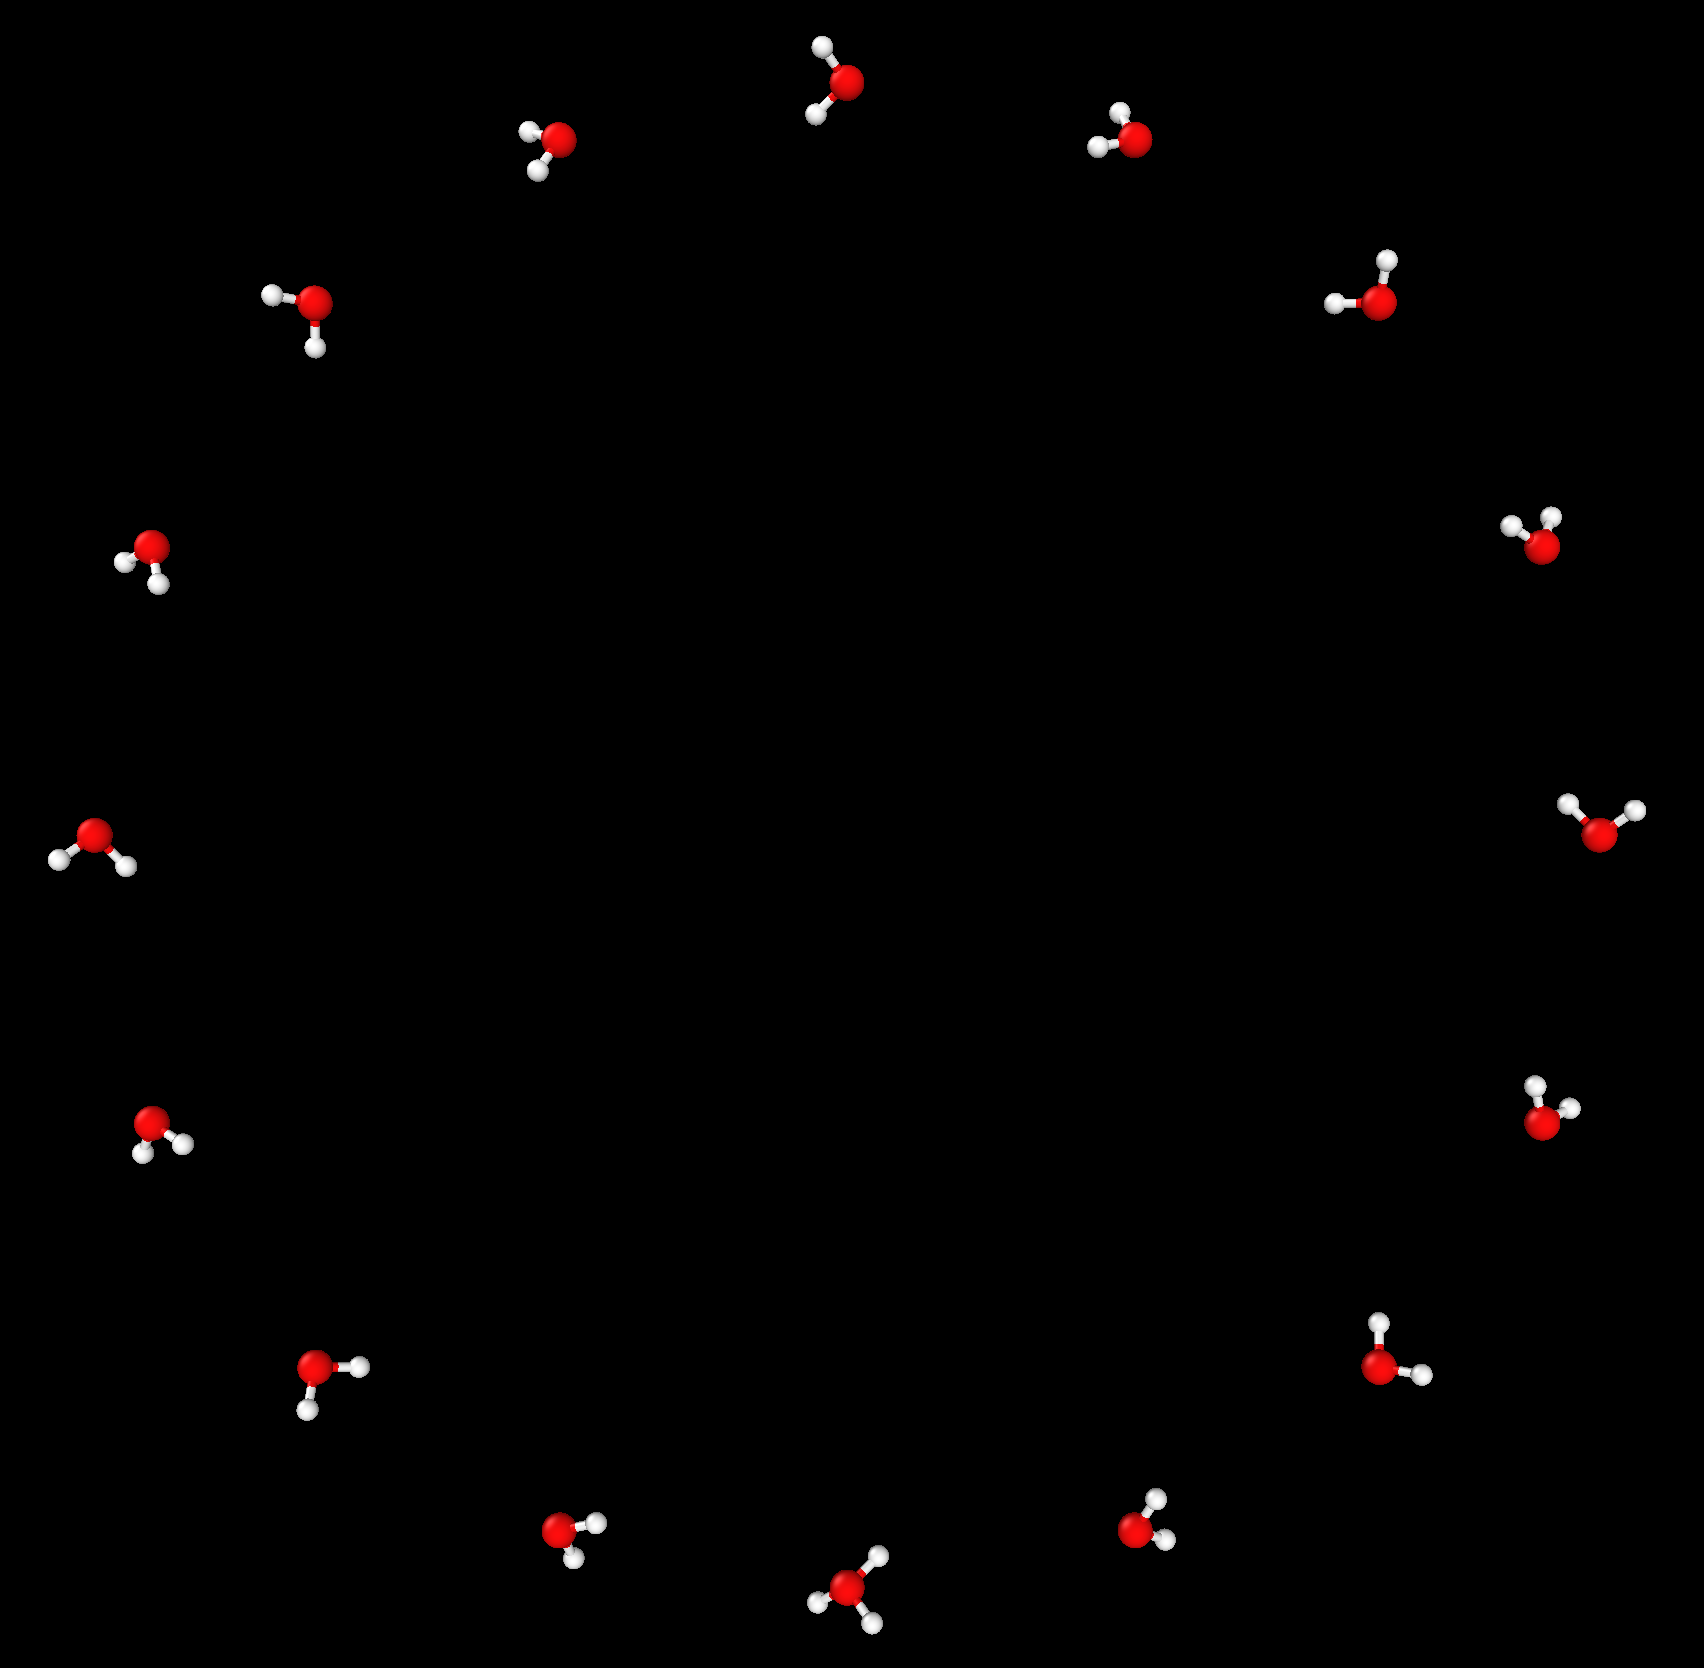
\includegraphics[width=0.9\textwidth]{figures/circle}
	\captionof{figure}{\textit{The cell containing 15 water molecules and a hydronium ion arranged in a ring. Oxygen atoms are coloured red and hydrogen atoms are coloured white.}}
	\label{fig:circle}	
\end{Figure}

Our next method was to create a ring of water molecules and then to change one of the molecules to a hydronium ion. The mass of the oxygen atoms was set to an arbitrary very large mass so that when we ran molecular dynamics simulations, the oxygen atoms would stay almost completely still. This would allow us to see the Grotthuss process in a simplified environment.

To do this I created a script which placed oxygen atoms at even intervals around the circumference. The distance between the oxygen atoms was specified and the radius of the circle was calculated using the formula,
\begin{equation}
	r=\frac{d_{\text{OO}}}{2\sin{\pi/n}}
\end{equation} 
where $d_\text{OO}$ is the distance between oxygen atoms and $n$ is the number of water molecules.

For each oxygen atom, we randomly generated two unit vectors in 3D space. These would create the plane on which the three atoms of each molecule would lie. First, we placed an hydrogen atom at a distance of 1.8141371 Bohr from the oxygen atom in the direction of the first vector. Next we took a cross product of the two randomly generated vectors and normalised it to create a unit vector normal to the molecular plane. Then we used the rotation matrix $R(\boldsymbol{\hat{\textbf{n}}},\theta)$ defined in \ref{sec:making_h3o+} to rotate the first vector by the bond angle of $104.5\degree$ and placed a second hydrogen atom at a distance of 1.8141371 Bohr from the oxygen atom in the direction of the new rotated vector.

Having done this for all the molecules, we relaxed the ring of water molecules using molecular statics, replaced one of the water molecules with a hydronium ion, then attempted to again relax the positions of the hydrogen atoms. 

At this stage we ran into a similar problem as in section \ref{sec:longbox} where TBE running in relaxation mode could not reach self consistency. This meant that running molecular dynamics would not be possible.

Having subsequently run molecular dynamics in bulk water, it is clear that using this method would not have been a good way to simulate the Grotthuss process. This is because the nuclei are treated as classical particles and as seen in figure \ref{fig:Zundel}, classical protons are highly unlikely to cross between molecules if the distance between the oxygen atoms is large. As this artificially fixed the positions of the oxygen atoms, the distance between them would never have been small enough to allow the protons to move between molecules.

\subsubsection{128 Water Molecule Box}
\label{sec:128}
Next we tried to start with an `off the shelf' water cell. We used a cubic cell of 128 water molecules that had been created using TBE. We replaced the central water molecule with a hydronium ion, and removed one of the hydrogens from a water molecule in one of the corners.

Then, we tried to relax this new cell using molecular statics, but TBE could not create a self consistent configuration.

\subsubsection{Artificial Ab Atom}
After some investigation, we discovered that the reason that the cell in section \ref{sec:128} was failing to reach self consistency was because TBE was finding two solutions for the number of electrons that the oxygen atom in the hydronium ion should have in its outer shell: eight and six. When trying to find self consistency, TBE would use one solution for a few steps and then switch, so it couldn't find a self-consistent solution to a high level of accuracy.
\begin{Figure}
	\centering
	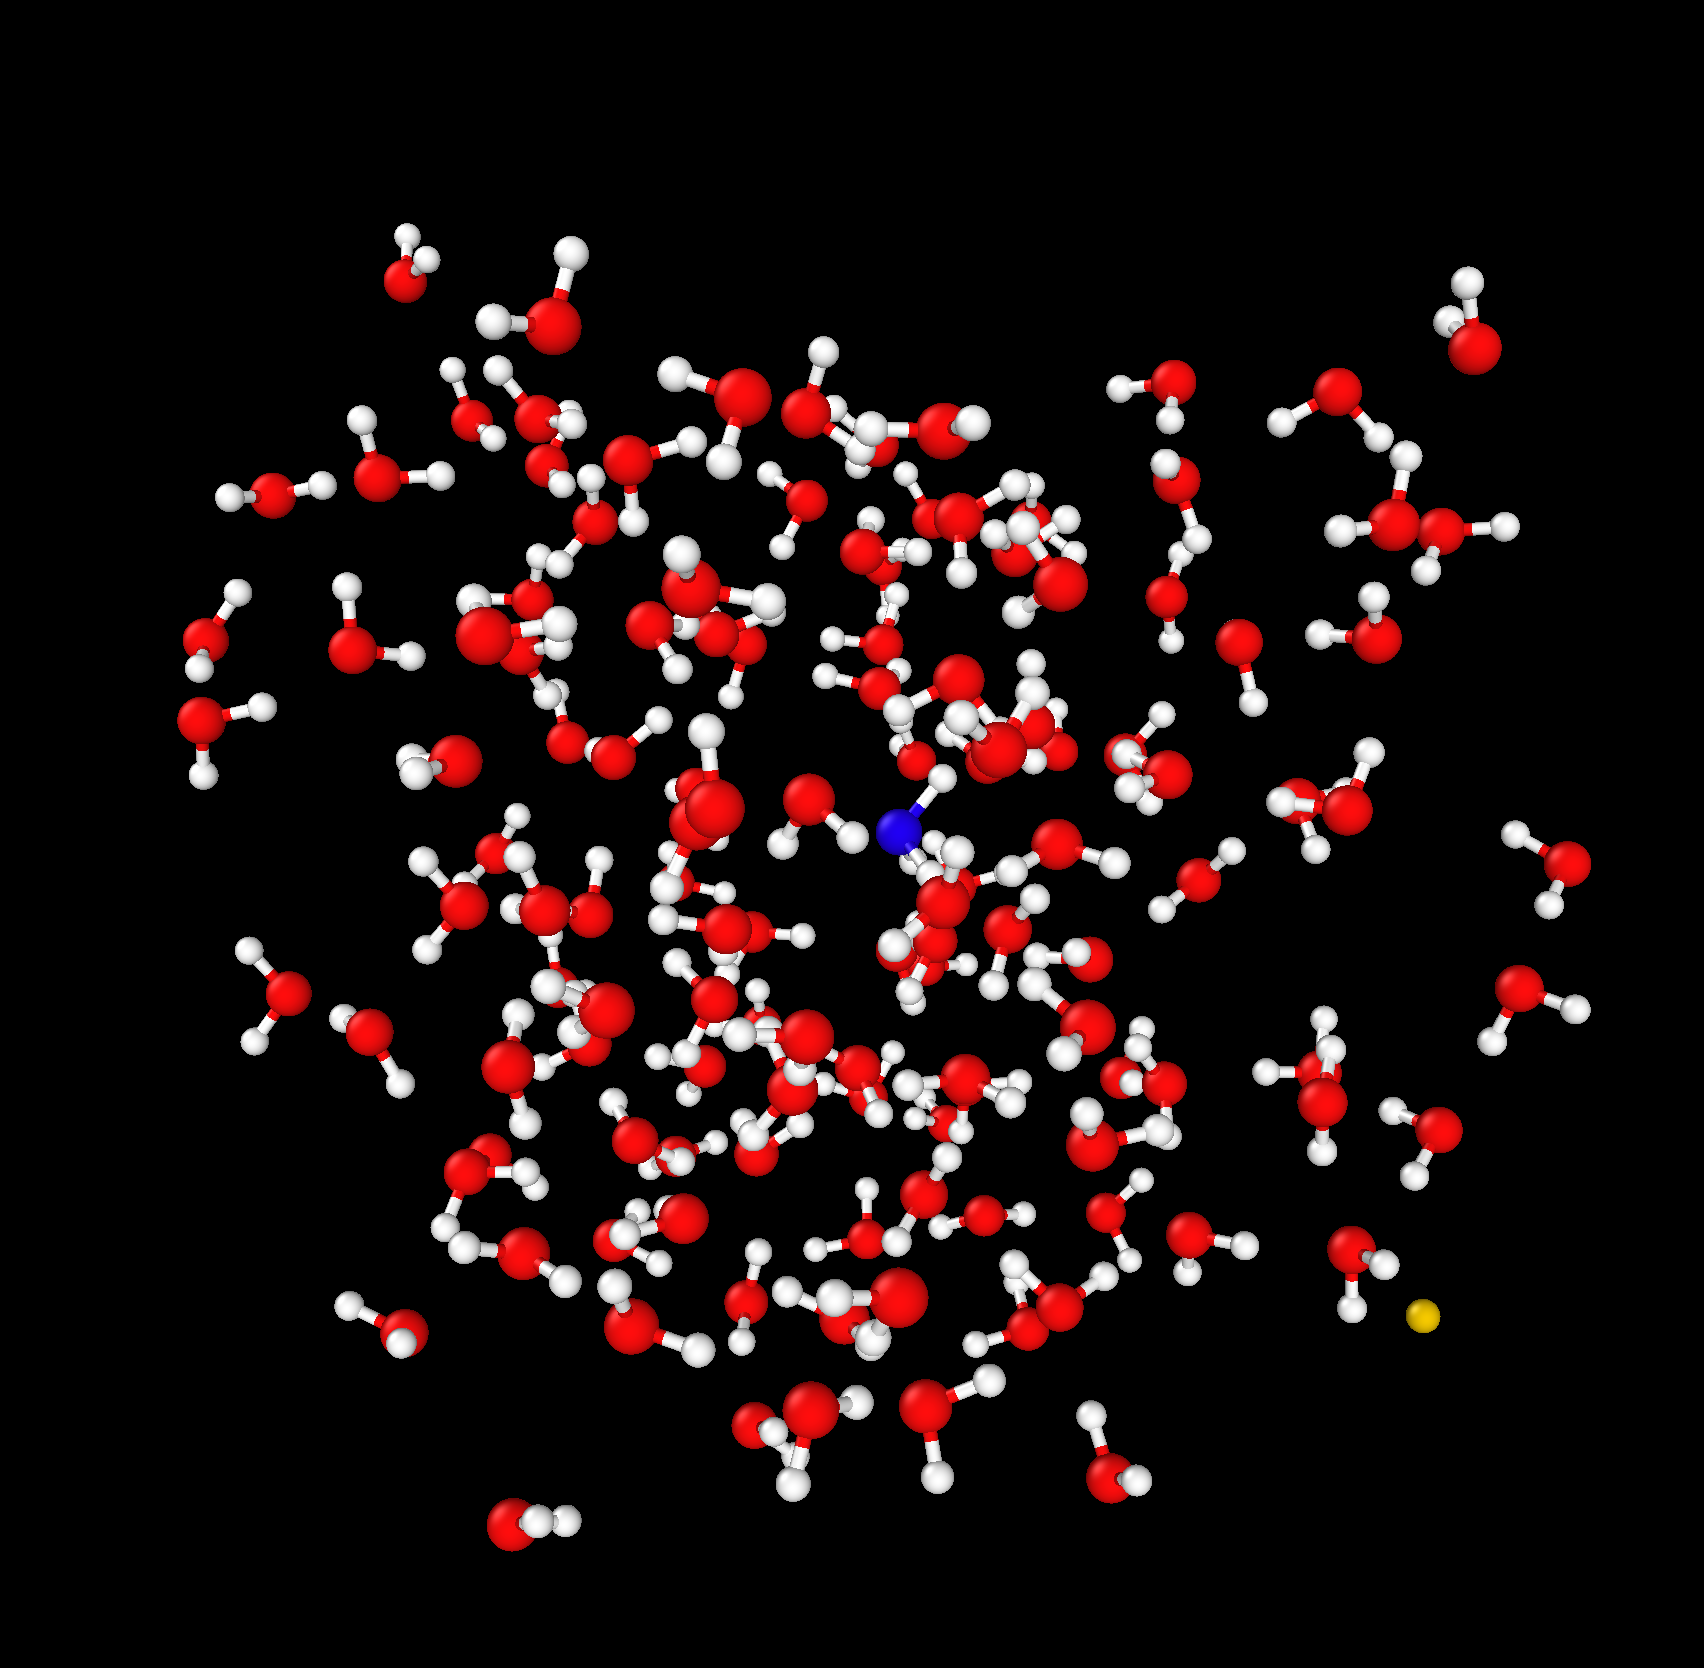
\includegraphics[width=0.9\textwidth]{figures/Ab}
	\captionof{figure}{\textit{The cell containing 126 water molecules, a hydronium ion and an Ab atom. The hydrogen atoms are all coloured white, the Ab is yellow, The oxygen in water molecules is red, and in the hydronium ion is blue.}}
	\label{fig:Ab}	
\end{Figure}

To solve this problem, we removed the hydroxide ion and replaced it with an artificial atom which we named Ab. This atom had a nucleus with charge $+1$ and was configured so that it would steal an electron and hold on to it so that it had a net charge of -1, allowing the hydronium to have the correct charge. 

To avoid the Ab atom interacting with other atoms, its matrix elements were all set to zero. To keep the other atoms at a distance, it had very large pair potentials with the other atoms.

This configuration converged during relaxation and produced stable molecular dynamics runs.

\subsubsection{Metal Mode}
\label{sec:metal}
\begin{Figure}
	\centering
	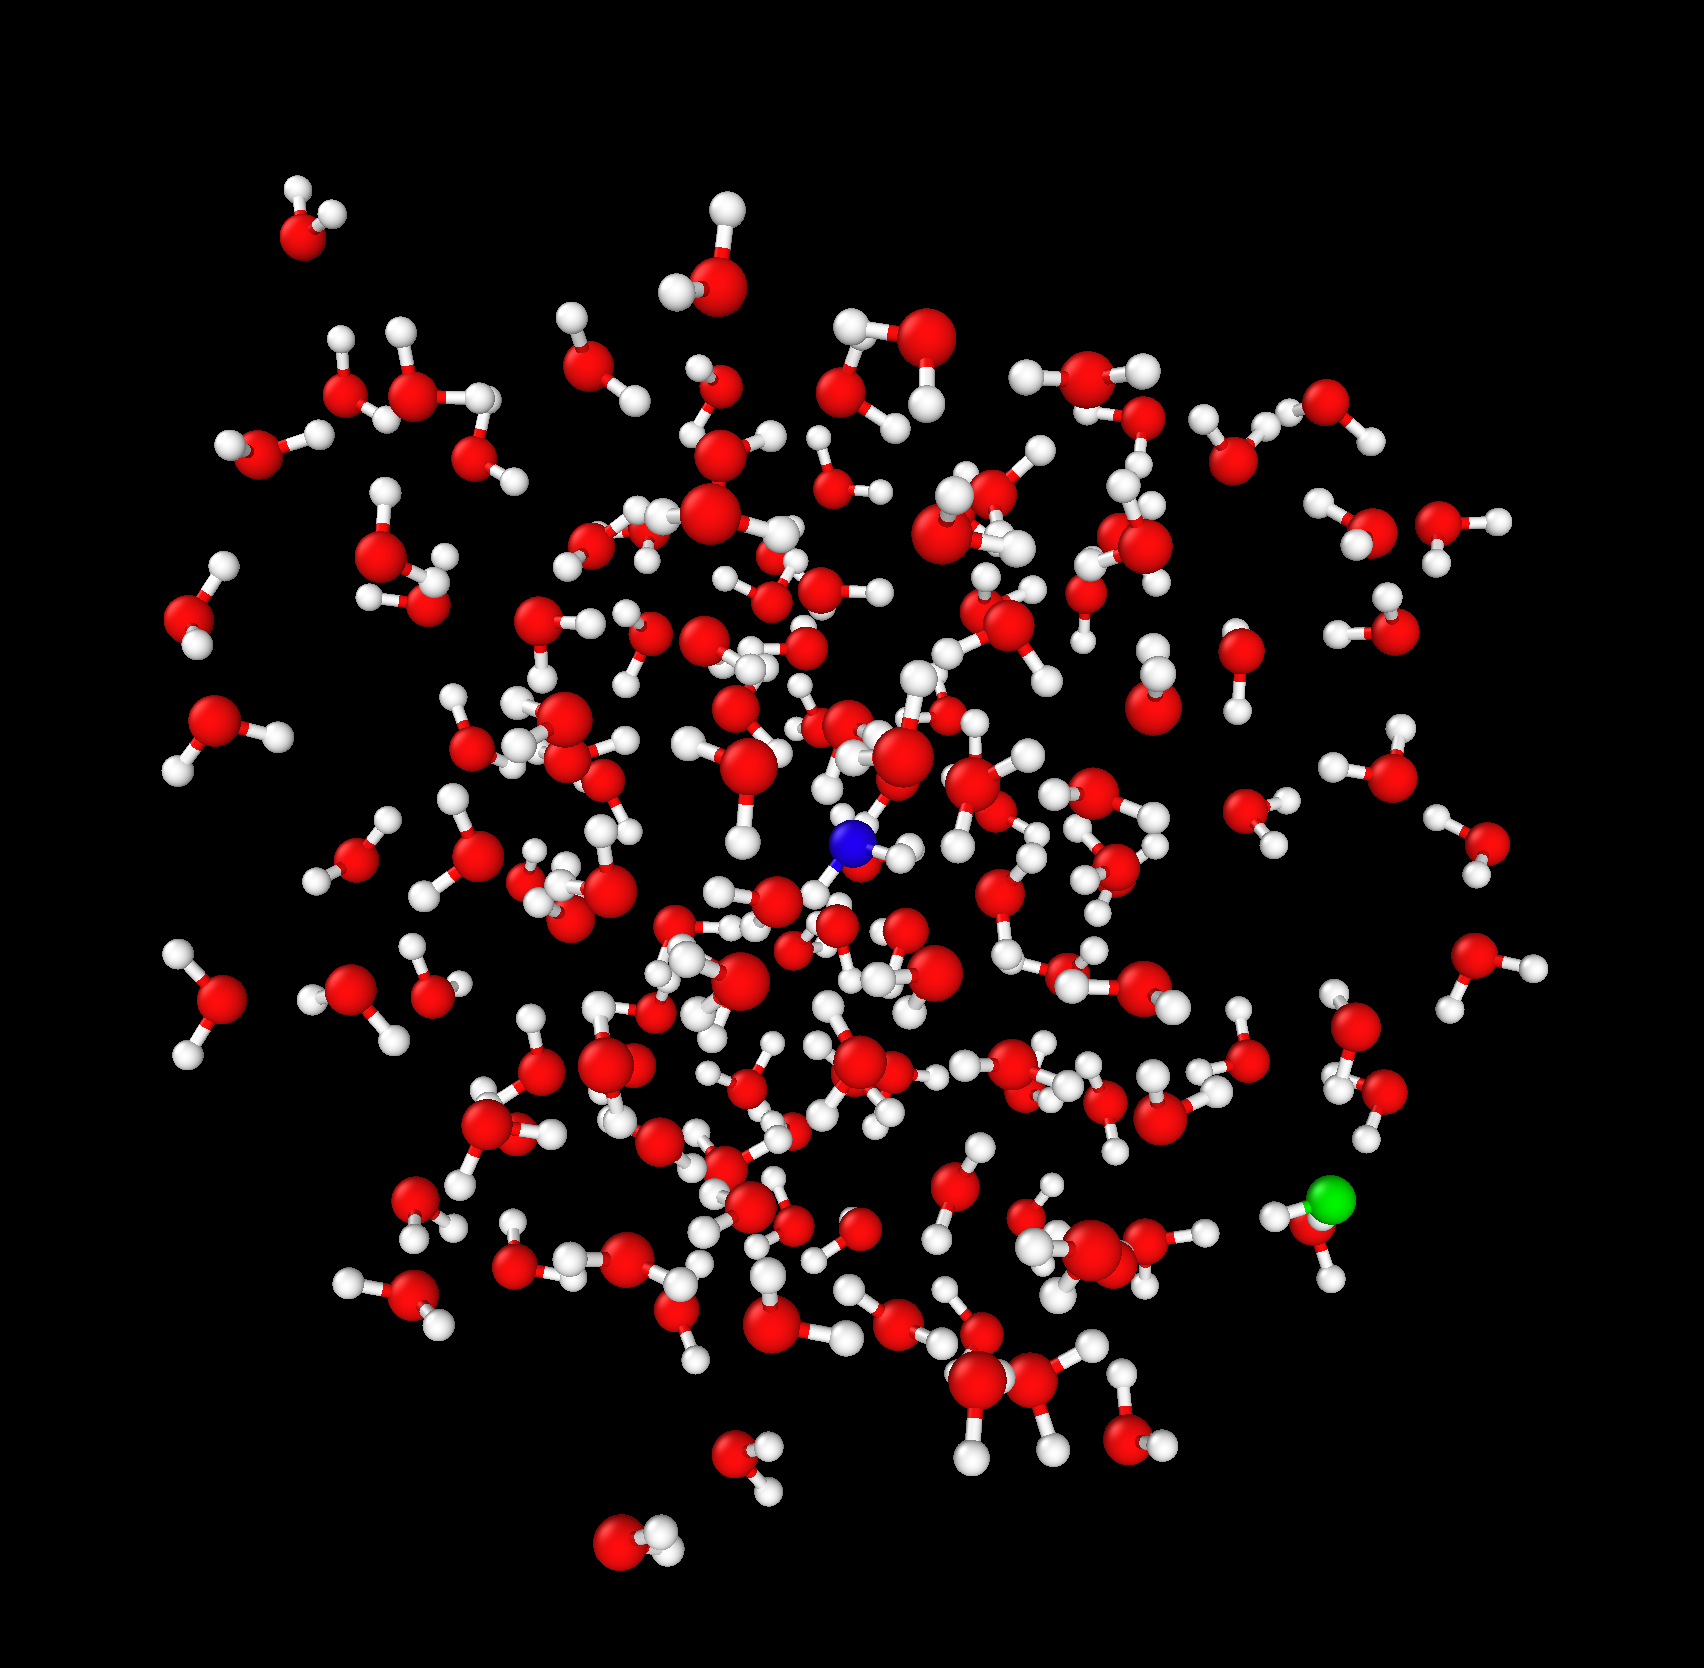
\includegraphics[width=0.9\textwidth]{figures/128}
	\captionof{figure}{\textit{The cell containing 126 water molecules, a hydronium ion and a hydroxide ion. The hydrogen atoms are all coloured white, the Ab is yellow. The oxygen in water molecules is red, in the hydronium ion is blue, and in the hydroxide ion is green.}}
	\label{fig:128}	
\end{Figure}

While working with the Ab atom above we solved the problem we were having in section \ref{sec:128} with regard to our OH\textsuperscript{-} ion not being self-consistent. We turned METAL mode on and increased W to 0.01. This allowed the code to overlap the two energy bands corresponding to the configurations. 
 
We ran molecular dynamics at a range of temperatures where water is a liquid i.e. between 273K and 373K.

\subsection{Analysing Simulations}
\label{sec:analysis}
TBE outputs xyz files which contain the species and coordinates for each atom at every time step in a molecular dynamics run. I wrote a python script which reads this file and calculates the distances between all the hydrogen and oxygen atoms at each step, taking into account that the closest distances may be through the periodic boundaries of the cell. The script then assigns each hydrogen to the oxygen it was closest to, before calculating the total number of hydrogens assigned to each oxygen. If this value is 3, the oxygen is relabelled O1 to indicate it is part of an H\textsubscript{3}O\textsuperscript{+} ion, and if it is 1 the oxygen is relabelled O2 to indicate it is part of an OH\textsuperscript{-} ion. If the value is 2 the oxygen is left as O. This makes it easier to differentiate between the ions in visualisation programs like Ovito.\cite{ovito}

The script then checks where O1 appears in the list and compares it to the previous step. If they differ, it adds 1 to the number of times a proton swapped molecule. If there is no O1, the script records that the H\textsubscript{3}O\textsuperscript{+} and OH\textsuperscript{-} ions have met, forming two water molecules, and the script stops.

Finally the script reads the MD file which records data for each time step, including the temperature. The script records all the temperatures before the ions meet and calculates the mean and standard deviation. The script outputs to a text file: the number of steps in the MD run, the number of proton swaps, the mean and standard deviation of the temperature,\footnote{We used the standard deviation in the temperature as an estimate for the error in the temperature.} and whether the ions meet. 

\section{Observations}

\subsection{Grotthuss Jumps}
A first and non-trivial observation is that in the tight binding Grotthuss simulations, Grotthuss jumps do occur and allow protons to be transferred throughout the body of water. Hydronium ions do not hold on to their extra proton, nor does it break away entirely from its surrounding water molecules and travel throughout the cell as a solitary atom.\footnote{This is with the caveat that in some situations the simulation breaks down and the proton does indeed break away from the water molecules.} Instead hydronium hydrogen bonds with the surrounding molecules and protons are transferred within these bonds.

\subsection{Flickering Events}
During molecular dynamics runs the majority of Grotthuss swaps were immediately followed by the proton swapping back to the original molecule. This was either because the proton that swapped molecules did so because of a particularly high kinetic energy, which is not immediately distributed to the other atoms in the new molecule; because of this, the proton is still likely to break away from the new molecule. Or it was because both molecules were aligned with their oxygen atoms facing towards the protons; as such, they both strongly attract the proton.

This means that the proton rapidly moved between the two molecules, gradually distributing its kinetic energy until the hydronium ion became stable.

This effect is, in essence, the two molecules becoming a Zundel cation \cite{Zundel2006} as described in section \ref{sec:cations}, where the two molecules came together and for a time, shared the proton via their hydrogen bond.

\subsection{Differences between H\textsubscript{3}O\textsuperscript{+} and OH\textsuperscript{-}}
We observed that, while the hydronium ion would perform many Grotthuss jumps, the hydroxide ion didn't undergo its equivalent process. This indicates that the potential barrier for a proton to move from a water molecule to a hydroxide ion is much higher than that for moving between a hydronium ion and a water molecule.\footnote{Recall that our simulation has classical particles. Zero-point energy and quantum tunnelling effects allow the protons to move from water molecules to hydroxide ions.} In hydronium there are three protons repelling each other compared to water's two. This means that a hydronium ion will have a higher potential energy meaning that it is more likely to perform a Grotthuss jump.

Despite our simulation treating protons as classical particles, our results mirror the experimental results found by Lee et al. in 2014 \cite{Lee2014} and the density functional theory simulations performed by Chen at al. \cite{chen2018hydroxide}. They observed that whilst H\textsubscript{3}O\textsuperscript{+} would diffuse via the Grotthuss process,  OH\textsuperscript{-} diffuses only by Brownian motion.

\subsection{Simulation Breakdown}
\label{sec:breakdown}
Simulations run at above 350K, which is the upper limit used in the paper that this tight binding model was taken from, \cite{Lozovoi2014}, have a high likelihood, as shown in figure \ref{fig:stability}, of breaking down in a way that isn't observed in real water.\cite{bell2013proton} A proton can break away from the hydronium ion if several oxygen atoms come close to it. However in this case, the protons gets suspended in between the water molecules, and instead of joining one of them to form a new hydronium ion, remains as a lone proton.
\begin{Figure}
	\centering
	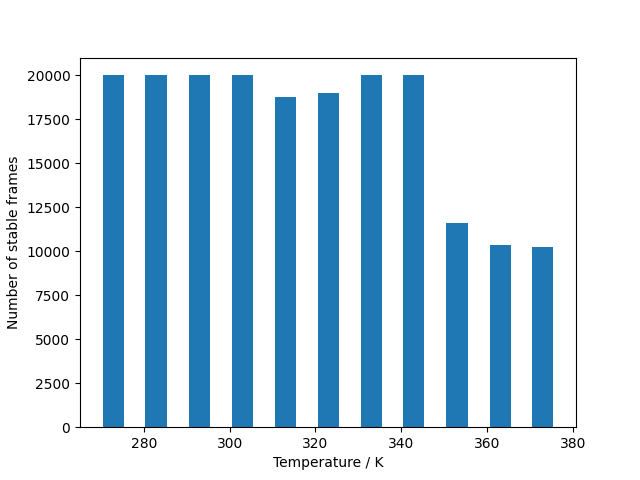
\includegraphics[width=0.9\textwidth]{figures/stability.png}
	\captionof{figure}{\textit{A bar chart showing how how many time steps a simulation ran before breaking down, up to a maximum of 20,000 steps,  against the mean temperature of the simulation.}}
	\label{fig:stability}	
\end{Figure}

This breakdown in our simulation meant that we had to reduce the time period where we were recording the temperature and number of Grotthuss swaps to just the period before the breakdown. We did this by making the code which analyses the xyz files stop if there is a hydrogen atom with no oxygen atoms within 1.92\AA\.footnote{This is roughly equal to 2 times the length of a typical H\textsubscript{2}O bond length.}

\section{Results}
\subsection{Jumping Rate}
\begin{Figure}
	\centering
	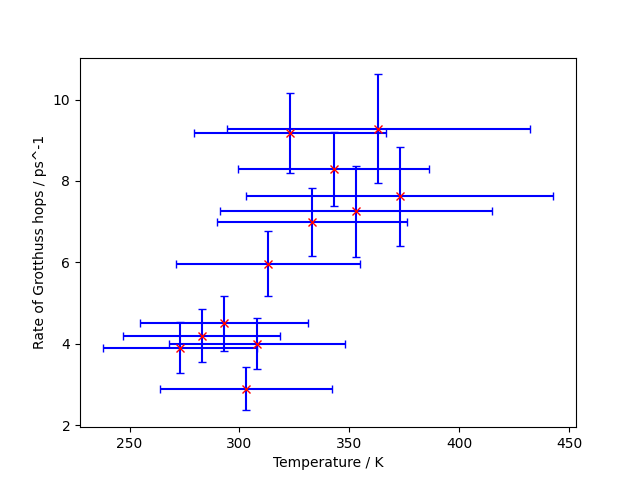
\includegraphics[width=0.9\textwidth]{figures/unscreeneddata.png}
	\captionof{figure}{\textit{The unscreened jumping rate of the hydronium ion is $ps^{-1}$ for a range of temperatures as described in section \ref{sec:metal}.}}
	\label{fig:unscreened}	
\end{Figure}

When plotting the jumping rate against temperature in figure \ref{fig:unscreened} we noticed that simulations which broke down had much higher average jumping rates than those at similar temperatures which didn't break down. This is because each simulation starts with a large number of jumps before settling in to a steadier, lower rate as shown in figure \ref{fig:histogram}, since the particular conditions of the simulations have undergone a sudden change and are now less stable for a short time. To compensate for this and give a more realistic figure for the jumping rate at each temperature, we ignored the first 1ps of the simulations, treating it as a screening period. The screened data is plotted in figure \ref{fig:screened}.
\begin{Figure}
	\centering
	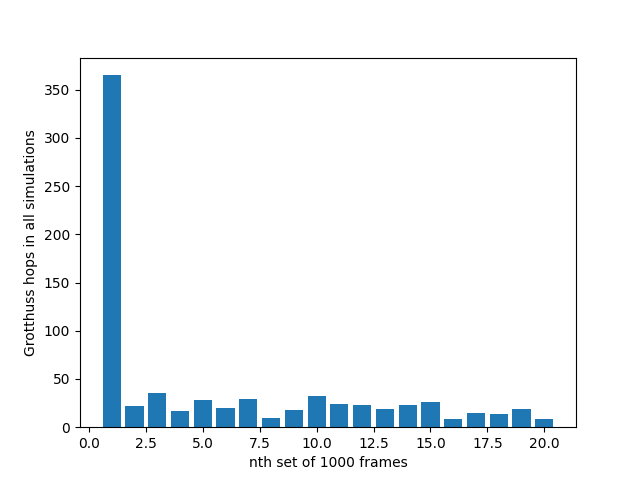
\includegraphics[width=0.9\textwidth]{figures/histogram.png}
	\captionof{figure}{\textit{A chart of the total number of jumps in the n\textsuperscript{th} set of 1000 time steps summed over all simulations.}}
	\label{fig:histogram}	
\end{Figure}

\begin{Figure}
	\centering
	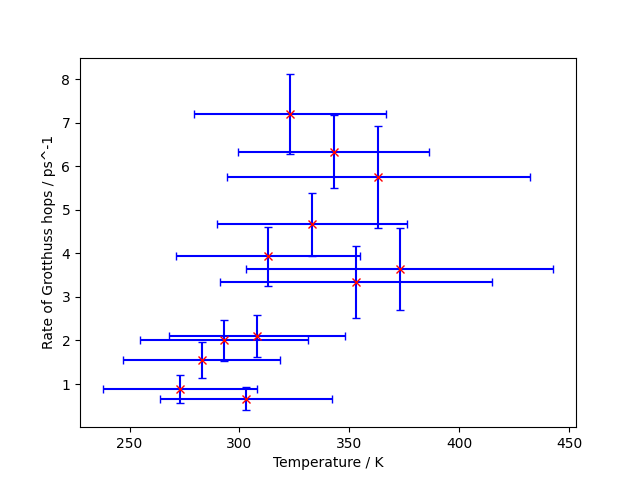
\includegraphics[width=0.9\textwidth]{figures/screeneddata.png}
	\captionof{figure}{\textit{The jumping rate of the hydronium ion in $ps^{-1}$ for a range of temperatures as described in \ref{sec:metal} with the first 2000 time steps screened out.}}
	\label{fig:screened}	
\end{Figure}
\subsubsection{Estimating Error in Jumping Rate}
To calculate an estimate of the error in the jumping rates, which we would use as our error bar, for each molecular dynamics simulation, we treated them as a binomial distribution where the set of all the time intervals\footnote{Excluding the first 2000 time intervals that we screened out.} are treated as a random sample. To calculate the standard deviation we used the formula
\begin{equation}
	\sigma=\sqrt{np(1-p)}
\end{equation}
where $n$ is the number of time steps and $p$ is the probability that a Grotthuss jump happens in any particular time step. $p$ was calculated by dividing the total number of Grotthuss jumps by the number of time steps.

\subsubsection{Estimating Temperature Dependence.}

To estimate the temperature dependence of the jumping rate we fitted the data to the Arrhenius equation \cite{arrhenius1889dissociationswarme}
\begin{equation}
	\label{eq:arrhenius}
	r = r_{0}\exp{\frac{-E_{A}}{k_{B}T}},
\end{equation}
where $r$ is the jumping rate, $r_0$ is a pre-exponential factor, $E_{A}$ is the activation energy of the reaction and $k_{B}$ is the Boltzmann constant.\cite{planck1900theory}

By taking the logarithm of equation \ref{eq:arrhenius} 
\begin{equation}
	\label{eq:logr}
	\log{r}= \log{r_{0}} -\frac{E_{A}}{k_{B}}\frac{1}{T}
\end{equation}
we can see that by plotting $\log r$ against $\frac{1}{T}$ we will get a straight line with a y-intercept of $\log r_{0}$ and a gradient of $-\frac{E_{A}}{k_{B}}$.

Using the method set out in reference \cite{gatland1993weight} we constructed a weighted least-squares best fit line where each point was given a weighting of 
\begin{equation}
	W_{i}=\frac{1}{{\sigma_{T}}^{2}+(\frac{\sigma_{r}}{r})^{2}}
\end{equation}
and calculated values of $2148.3607\text{ps}^{-1}$ for $r_{0}$ and $2098.0025$ K for $\frac{E_{A}}{k_{B}}$.
\begin{Figure}
	\centering
	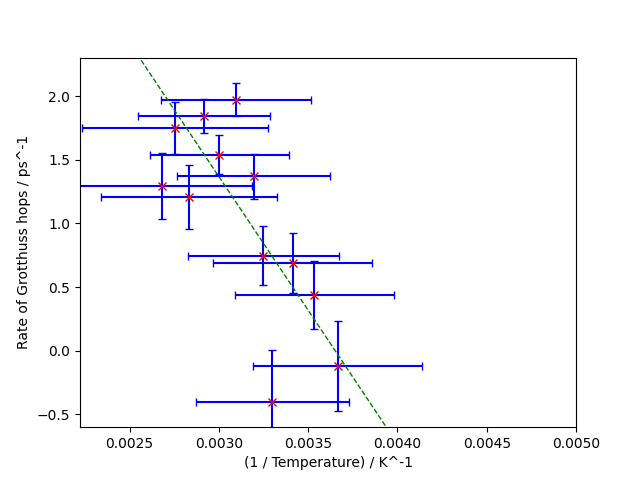
\includegraphics[width=0.9\textwidth]{figures/bestfitline.png}
	\captionof{figure}{\textit{The natural logarithm of the jumping rate of the hydronium ion plotted against $1/$temperature with a weighted best fit line plotted through it according to equation \ref{eq:logr}.}}
	\label{fig:bestfitline}	
\end{Figure}

By returning the axes to linear ones, we plotted our data superimposed on the best fit curve as shown in figure \ref{fig:bestfitcurve}.

\begin{Figure}
	\centering
	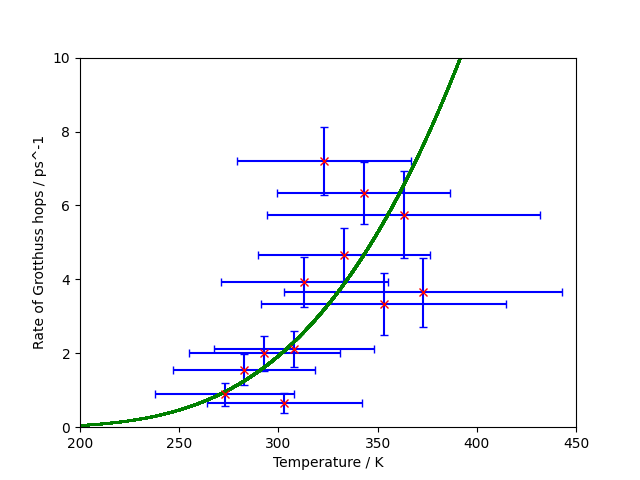
\includegraphics[width=0.9\textwidth]{figures/bestfitcurve.png}
	\captionof{figure}{\textit{The jumping rate of the hydronium ion in $ps^{-1}$ for a range of temperatures as described in \ref{sec:metal} with the first 2000 time steps screened out. A weighted best fit curve is plotted through the data according to equation \ref{eq:arrhenius}.}}
	\label{fig:bestfitcurve}	
\end{Figure}
We estimated the error in  $r_0$ using the equation
\begin{equation}
	\frac{\sigma_{r_{0}}}{r_{0}}=\text{mean}\bigg(\frac{\sigma_{r}}{r}\bigg)
\end{equation}
and estimated the error in $E_{A}$ as 
\begin{equation}
	\frac{\sigma_{E_{A}}}{E_{A}}=\sqrt{\bigg(\text{mean}\bigg(\frac{\sigma_{r}}{r}\bigg)\bigg)^{2} + \bigg(\text{mean}\bigg(\frac{\sigma_{T}}{T}\bigg)\bigg)^{2}}.
\end{equation}
Putting this all together and using the Boltzmann constant in electron volts per Kelvin, we calculate that the activation energy of a Grotthuss jump is $0.1808\pm 0.0496$ eV and the Grotthuss jumping rate of a hydronium ion in water is 
\begin{equation}
	\label{eq:result}
	(2184.36 \pm 509.17)\exp{-\frac{2098.00 \pm 576.80}{T}} \text{ps}^{-1}.
\end{equation}
\section{Discussion}
Although the errors in our results are large ($\sigma_{r_{0}}\approx 22\%$ and $\sigma_{E_{A}}\approx 26\%$), the process was modelled well at most lower temperatures as evidenced in figure \ref{fig:bestfitcurve}, with the exception of the anomalously low rate at 303K. Curiously, the three simulations that were run above this temperature range not only broke down, but also had jumping rates below the best fit curve.

However, even though the higher temperature results are not as accurately described by equation \ref{eq:result}, the best fit curve still passes through the error bars of all but one point. This is good evidence that equation \ref{eq:result} is a valid model for the jumping rate in our simulation.

This method would definitely benefit from having much more data, both longer MD runs and at more temperatures. These would provide much more accurate estimates of $E_{A}$ and $r_0$. 

Unfortunately, the method for calculating the error in a linear fit by calculating $\chi^2$ as described in reference \cite{gatland1993weight} is not appropriate for our method of weighting as we had errors in both the $x$ and $y$ axes. For future work we should use fitting methods that allow us to calculate errors in $E_{A}$ and $r_0$ that reduce as we add more points, akin to the way that the error on the mean of values, taken from a distribution, reduces as the number of values increases. Our crude calculations of $\sigma_{r_{0}}$ and $\sigma_{E_{A}}$ do not.

\section{Opportunities for Future Research}

\subsection{Changes to Current Model}
To allow for longer molecular dynamics simulations which would produce more accurate results, investigation into the cause of the simulation break down described in section \ref{sec:breakdown} would be necessary. Altering the model taken from source \cite{Lozovoi2014} so that it mirrors the property of real water, whereby protons cannot exist in a solitary fashion,\cite{bell2013proton} but instead covalently bond to water molecules to form hydronium ions, would allow the simulations to run for hundreds of picoseconds. This would allow measuring the time for hydroxide and hydronium to meet.

\subsection{Water Wire}
An alternative to the flat ring described in section \ref{sec:ring} would be to create a water wire in three dimensions joined at both ends where the angle between every set of three consecutive molecules is $109.5^{\circ}$.\footnote{This is the angle between particles arranged in a tetrahedral lattice.} This is equivalent to taking an ice lattice and removing all the molecules apart from the ones ones that make up the wire. Stationary molecules that imitate water, may have to be arranged around the wire (to form stationary hydrogen bonds with the lone pairs on the oxygen atoms in the chain) to improve the simulation.

This would have the advantage of keeping the hydrogen bonds nearly straight and therefore possibly allowing the Grotthuss process to occur more easily.

\subsection{Quantum Simulation}
\label{sec:PIMD}
Whilst the calculations that TBE performs are quantum mechanical in nature, in molecular dynamics the atomic nuclei themselves move as classical particles. For light nuclei, like hydrogen, this is a poor approximation as the effect of zero-point energy\footnote{The zero-point energy is the lowest energy state a system can exist in. Figure \ref{fig:Zundel} provides a good visualisation of how the zero-point energy affects the way a proton behaves in the Grotthuss process. When comparing the two low temperature simulations we notice that the classical simulation has a very narrow distribution, whereas in the quantum simulation the proton has a much wider distribution. This is because in the quantum simulation the proton has a minimum energy at very low temperatures and therefore can be in positions further from the equilibrium line. In contrast, the energy of a classical particle tends to zero as the temperature tends to zero and so the particle stays very close to the equilibrium line at low temperatures.} and quantum tunnelling will be large. To take into account these effects we can use a technique called path integral molecular dynamics (PIMD).\cite{Feynman1965,Feynman1948,Gillan1990}

This would be especially useful for simulations like the ring described in section \ref{sec:ring} as it would allow protons to quantum tunnel between molecules without needing the oxygen atoms to move. Assuming that a solution for the problems with finding self-consistency when using TBE can be found, having the molecules arranged in a ring with the oxygen atoms artificially held still would be a way to very clearly show the difference between TBE's MD and the PIMD in I-Pi, in TBE the protons would have a very low jumping rate as the molecules can't move and a proton can only move between molecules on the very rare occasion that it has enough energy to break away from the hydronium ion. In contrast, using I-Pi; the protons would have a probability of tunnelling to an adjacent molecule. This can happen at lower energy as explained in figure \ref{fig:tunnelling} and therefore would have a much higher probability of happening.

\begin{Figure}
	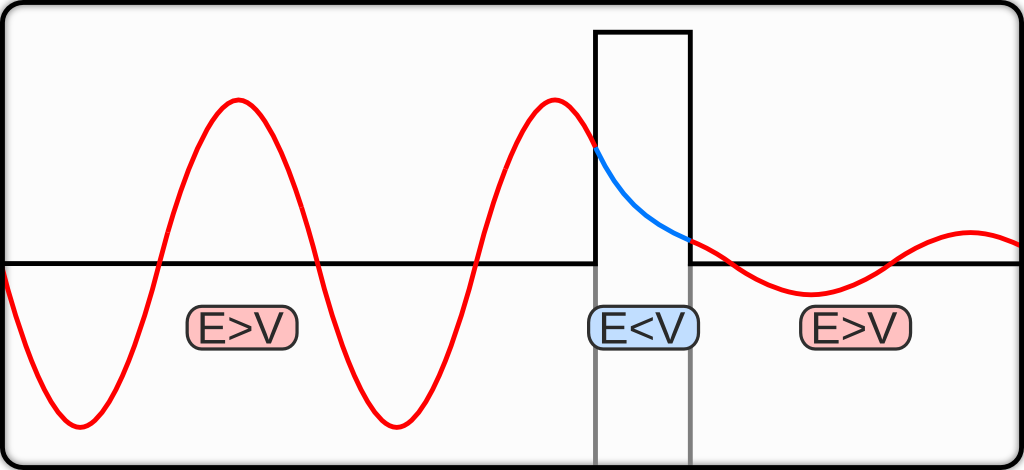
\includegraphics[width=\textwidth]{figures/tunneling.png}
	\captionof{figure}{\textit{A diagram of a simple one dimensional system showing a wave function with energy $E$ tunnelling through a barrier}.\cite{decross_ellinor_film}\textit{ This system is analogous to how a proton would behave under PIMD, with the potential well on the left being the hydronium ion and the well on the right being a water molecule. The empty space in between the two molecules is represented by the potential barrier. Notably we can see how the wave function can tunnel through the barrier even though the barrier has potential $V>E$. Under TBE the analogous system is one in which a classical particle with kinetic energy $E$ encountering a barrier with potential $V$. In this system the particle can only pass the barrier if $E>V$, otherwise the particle is reflected back. This figure was taken from \cite{Tunneling}.}}
	\label{fig:tunnelling}	
\end{Figure}

\subsection{Diffusivity Calculation}
Creating larger cells of water and running simulations that are stable for long periods of time\footnote{Simulations that can last for several hundred picoseconds would be ideal for this.} would allow us to track the rate at which hydronium ions move away from their initial positions. This would allow us to calculate the diffusivity of the hydronium ions in bulk water.

\subsection{Applied Potential Difference}
Though this would require serious modifications to the way TBE and the related Questaal codes work, it would be interesting to try to create a mechanism whereby the Grotthuss process in the presence of an electric field could be observed. Perhaps two opposing faces of the cell could be used as a barrier that repels oxygen atoms but encourages hydrogen atoms to pass through in one direction.

A system which could create this effect would allow you to observe the rotating stage of the Grotthuss mechanism which isn't really observed in our random process.

\subsection{Conductivity of Water}
Following on from the previous section. Creating a system in which a potential difference across the cell induces a current, would allow for a calculation of the conductivity. We would not be able to create a cell with enough water molecules per hydronium to calculate this value directly,\footnote{See section \ref{sec:autoprotonation}.} but calculating the conductivity for a range of different sizes of cell would allow us to extrapolate an estimate for the conductivity of water which we could compare to experimental results.\cite{Rodger1894}

\subsection{Comparison to Hydrogen Fluoride or Liquid Ammonia}
Hydrogen fluoride and ammonia molecules can also both donate and receive protons, as well as both featuring hydrogen bonding and can auto-protonate to form fluoride and fluoronium ions, and amide and ammonium ions respectively. They could therefore also have their own process equivalent to the Grotthuss process. It would be interesting to test the effect  having different numbers of lone pairs and protons has on the process. Indeed liquid hydrogen fluoride may act much like the OH water that Grotthuss mistakenly described in his original paper.\cite{Grotthuss1805}

\section{Conclusions}
In conclusion, our tight binding model for water does successfully simulate the Grotthuss process, allowing proton transfer throughout a body of water. 

Our model produces stable molecular dynamics simulations that can last for at least 10ps for temperatures below 350K but break down at higher temperatures.

The activation energy of a Grotthuss jump is $0.1808 \pm 0.0496$ eV and the rate at which a proton jumps from one molecule to another is given by the formula $(2184.36 \pm 509.17)\exp{-\frac{2098.00 \pm 576.80}{T}} \text{ps}^{-1}$.


\bibliography{GrotthussBibliography} 
	\bibliographystyle{ieeetr}
\end{multicols}
\end{document}